% !TeX program = xelatex
\documentclass[a4paper,10pt]{article}

% ============================================================================
% កញ្ចប់សម្ភារៈសិក្សាបោះពុម្ព ស-ខ្មៅ (Printable Classroom Materials - Grade 8 HA)
% ត្រូវគ្នា ១០០% នឹង LS_Plan_HA.tex និង Teaching_Scenario_HA.tex
% ============================================================================
\usepackage[a4paper, left=1.0cm, right=1.0cm, top=0.75cm, bottom=1.05cm, footskip=0.55cm]{geometry}
\usepackage{amsmath, amssymb}
\usepackage{unicode-math}
\usepackage{fontspec}
\usepackage{array, colortbl}
\usepackage[table]{xcolor}
\usepackage{enumitem}
\usepackage{pifont}
\usepackage{fancyhdr}
\usepackage{lastpage}
\usepackage{tikz}
\usepackage[most]{tcolorbox}
\usetikzlibrary{calc, arrows.meta, angles, quotes, decorations.markings, babel}

% LaTeX 2025 compatibility guard
\makeatletter
\let\@expl@@@mark@update@singlecol@structures@@\relax
\makeatother

% ============================================================================
% ការកំណត់ពុម្ពអក្សរផ្លូវការ (Word-Styled Khmer + Cambria Math + Times New Roman)
% ============================================================================
% Cross-platform font path resolver (Windows local + Linux/Cloud repo fonts/)
\providecommand{\NGSFindFonts}{%
  \IfFileExists{C:/Windows/Fonts/cambria.ttc}{%
    \def\NGSSysPath{C:/Windows/Fonts/}%
    \def\NGSUserPath{C:/Users/KIT/AppData/Local/Microsoft/Windows/Fonts/}%
  }{%
    \IfFileExists{./fonts/KhmerOSsiemreap.ttf}{\def\NGSSysPath{./fonts/}\def\NGSUserPath{./fonts/}}{%
    \IfFileExists{../fonts/KhmerOSsiemreap.ttf}{\def\NGSSysPath{../fonts/}\def\NGSUserPath{../fonts/}}{%
    \IfFileExists{../../fonts/KhmerOSsiemreap.ttf}{\def\NGSSysPath{../../fonts/}\def\NGSUserPath{../../fonts/}}{%
    \IfFileExists{../../../fonts/KhmerOSsiemreap.ttf}{\def\NGSSysPath{../../../fonts/}\def\NGSUserPath{../../../fonts/}}{%
    \IfFileExists{../../../../fonts/KhmerOSsiemreap.ttf}{\def\NGSSysPath{../../../../fonts/}\def\NGSUserPath{../../../../fonts/}}{%
    \IfFileExists{../../../../../fonts/KhmerOSsiemreap.ttf}{\def\NGSSysPath{../../../../../fonts/}\def\NGSUserPath{../../../../../fonts/}}{%
    \IfFileExists{../../../../../../fonts/KhmerOSsiemreap.ttf}{\def\NGSSysPath{../../../../../../fonts/}\def\NGSUserPath{../../../../../../fonts/}}{%
      \def\NGSSysPath{../../../../../../../fonts/}\def\NGSUserPath{../../../../../../../fonts/}%
    }}}}}}}%
  }%
}
\NGSFindFonts

\setmathfont[
  Path={\NGSSysPath},
  FontIndex=1,
  Scale=1.02
]{cambria.ttc}

\defaultfontfeatures{Ligatures=TeX}

\setmainfont[
  Path={\NGSUserPath},
  Extension=.ttf,
  Script=Khmer,
  BoldFont={KhmerOSsiemreap},
  BoldFeatures={FakeBold=1.8},
  ItalicFont={KhmerOSsiemreap},
  ItalicFeatures={FakeSlant=0.25},
  BoldItalicFont={KhmerOSsiemreap},
  BoldItalicFeatures={FakeBold=1.8, FakeSlant=0.25}
]{KhmerOSsiemreap}

\newfontfamily\muol[
  Path={\NGSUserPath},
  Extension=.ttf,
  Script=Khmer
]{KhmerOSmuollight}

\newfontfamily\TimesEn[
  Path={\NGSSysPath},
  Extension=.ttf,
  BoldFont={timesbd},
  ItalicFont={timesi},
  BoldItalicFont={timesbi}
]{times}

\newfontfamily\CalibriFont[
  Path={\NGSSysPath},
  Extension=.ttf
]{calibri}

\newfontfamily\Tacteing[
  Path={\NGSUserPath}
]{TACTENG.TTF}

\XeTeXlinebreaklocale "km"
\XeTeXlinebreakskip = 0pt plus 1pt minus 0.1pt

% ============================================================================
% ក្ដារពណ៌ ស-ខ្មៅ សុទ្ធសម្រាប់ការបោះពុម្ព (Strict Monochrome Print Palette)
% ============================================================================
\definecolor{panelgray}{gray}{0.92} % ~gray!8
\definecolor{headgray}{gray}{0.85}  % ~gray!15
\definecolor{midgray}{gray}{0.75}   % ~gray!25
\definecolor{darkline}{gray}{0.35}  % ~gray!65

\pagestyle{fancy}
\fancyhf{}
\renewcommand{\headrulewidth}{0pt}
\fancyfoot[L]{\fontsize{8pt}{10pt}\selectfont អនុវិទ្យាល័យព្រះក្រសាំង \en{---} គណិតវិទ្យា ថ្នាក់ទី៨ \en{|} មេរៀនទី១២ (១.៣.១) ករណី អ.ម (\en{HA}) \& ពុះមុំ (ស-ខ្មៅ) \en{|} ថ្ងៃសៅរ៍ ទី២៨ ខែវិច្ឆិកា ឆ្នាំ២០២៦}
\fancyfoot[R]{\fontsize{8.5pt}{10pt}\selectfont ទំព័រ \en{\thepage\ / \pageref{LastPage}}}

\setlength{\parindent}{0pt}
\setlength{\parskip}{0pt}
\setlength{\tabcolsep}{4pt}

% ============================================================================
% ម៉ាក្រូជំនួយ (Helper Macros)
% ============================================================================
\newcommand{\en}[1]{{\TimesEn #1}}
\newcommand{\enbf}[1]{{\TimesEn\bfseries #1}}
\newcommand{\unit}[1]{\,\text{\en{#1}}}
\newcommand{\cnum}[1]{\mbox{\fontsize{10pt}{12pt}\selectfont\ding{\numexpr181+#1\relax}}}
\newcommand{\scissors}{\ding{34}}
\newcommand{\chkbox}{\tikz[baseline=-0.15ex]\draw[black, line width=0.85pt] (0,0) rectangle (0.25cm,0.25cm);}
\newcommand{\tickone}{\tikz[baseline=-0.2ex]\draw[black, line width=1.1pt] (0,0) -- (0,0.24cm);}
\newcommand{\ticktwo}{\tikz[baseline=-0.2ex]{\draw[black, line width=1.1pt] (0,0) -- (0,0.24cm);\draw[black, line width=1.1pt] (0.075cm,0) -- (0.075cm,0.24cm);}}
\newcommand{\tri}[1]{\ensuremath{\triangle #1}}
\newcommand{\ang}[1]{\ensuremath{\angle #1}}
\newcommand{\cg}{\ensuremath{\cong}}
\newcommand{\ncg}{\ensuremath{\not\cong}}
\newcommand{\khmflourish}{{\Tacteing\fontsize{30pt}{12pt}\selectfont\raisebox{-4pt}{3}}}

\newcommand{\pagebanner}[2]{%
  \begin{tcolorbox}[
    enhanced, sharp corners, colback=headgray, colframe=black,
    boxrule=1.1pt, boxsep=1pt, top=3pt, bottom=3pt, left=6pt, right=6pt,
    after skip=4pt
  ]
    {\muol\fontsize{9.6pt}{14pt}\selectfont #1}\hfill{\fontsize{8.0pt}{11.5pt}\selectfont\textbf{#2}}
  \end{tcolorbox}%
}

\newcolumntype{L}[1]{>{\raggedright\arraybackslash}p{#1}}
\newcolumntype{C}[1]{>{\centering\arraybackslash}p{#1}}

% Bold B&W Tick marks (>=1.0pt print safe) & Right-Angle box
\tikzset{
  tk1/.style={postaction={decorate},decoration={markings,
    mark=at position 0.50 with {\draw[black, line width=1.05pt] (0,-0.11)--(0,0.11);}}},
  tk1low/.style={postaction={decorate},decoration={markings,
    mark=at position 0.72 with {\draw[black, line width=1.05pt] (0,-0.10)--(0,0.10);}}},
  tk2/.style={postaction={decorate},decoration={markings,
    mark=at position 0.44 with {\draw[black, line width=1.05pt] (0,-0.11)--(0,0.11);},
    mark=at position 0.56 with {\draw[black, line width=1.05pt] (0,-0.11)--(0,0.11);}}},
  hypArrow/.style={black, densely dashed, line width=0.95pt, -{Stealth[length=1.7mm]}}
}

\begin{document}
\fontsize{9.0pt}{13.2pt}\selectfont

% ============================================================================
% ទំព័រទី ១៖ សម្ភារៈ E2 ខ្នាតពិត 1:1 (កែង 90° + 5 cm + 35° + POE 2A + POE 2B)
% ============================================================================
\pagebanner{សម្ភារៈទី ១៖ បន្ទះកាត់ \enbf{E2} ខ្នាត \enbf{1:1} កែង \enbf{90}$^\circ$ \enbf{\&} បត់កន្លះពុះមុំ}{ទំព័រ ១/៦ \en{-- E2 Explore}}

% --- ប្រអប់ព្រមានខ្នាតពិត & បន្ទះផ្ទៀង 5 cm (x=1cm, y=1cm) ---
\noindent
\begin{minipage}[c]{11.9cm}
  \begin{tcolorbox}[
    enhanced, sharp corners, colback=panelgray, colframe=black,
    boxrule=1.0pt, boxsep=1pt, top=3.5pt, bottom=3.5pt, left=6pt, right=6pt
  ]
    \fontsize{8.3pt}{11.8pt}\selectfont
    \textbf{ការណែនាំសំខាន់មុនបោះពុម្ព (\en{Actual Size 100\%})៖} ពេលបោះពុម្ព ត្រូវជ្រើស \textbf{\en{Scale: Actual Size 100\%}} \en{--} \textbf{កុំជ្រើស \en{Fit to Page}} ដើម្បីឱ្យអ៊ីប៉ូតេនុស $5\unit{cm}$, ជ្រុង $\approx 6.1\unit{cm}$, មុំ $35^\circ$, កែង $90^\circ$ និងទម្រង់បត់ $\ang{XOY}$ ត្រូវតាមខ្នាតពិត \en{1:1}។\\[1.5pt]
    \textbf{វិធីរៀបចំ (ក្រុមស្ថាបត្យករជណ្ដើរសុវត្ថិភាព)៖} កាត់តាមស្នាមចុច \scissors{} បង្វិលផ្ទៀងត្រួត និងបត់តាមបន្ទាត់ $OM$។
  \end{tcolorbox}
\end{minipage}%
\hfill
\begin{minipage}[c]{6.8cm}
  \begin{tcolorbox}[
    enhanced, sharp corners, colback=white, colframe=black,
    boxrule=1.0pt, boxsep=1pt, top=3pt, bottom=3pt, left=4pt, right=4pt
  ]
    \centering
    {\fontsize{8.0pt}{10.5pt}\selectfont\textbf{បន្ទះផ្ទៀងខ្នាតពិត \en{5 cm} (\en{Actual Size 100\% Check})}}\\[2pt]
    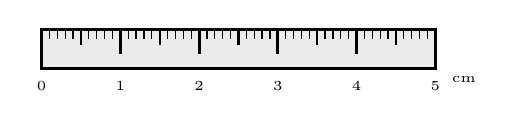
\begin{tikzpicture}[x=1cm, y=1cm, every node/.style={font=\scriptsize, text=black}]
      \draw[black, line width=1.1pt, fill=panelgray] (0,0) rectangle (5.0, 0.50);
      \foreach \m in {0,...,50}{
        \pgfmathsetmacro{\xval}{\m*0.1}
        \draw[black, line width=0.45pt] (\xval, 0.50) -- (\xval, 0.38);
      }
      \foreach \h in {0,0.5,...,5.0}{
        \draw[black, line width=0.8pt] (\h, 0.50) -- (\h, 0.30);
      }
      \foreach \c in {0,1,2,3,4,5}{
        \draw[black, line width=1.1pt] (\c, 0.50) -- (\c, 0.19);
        \node[below=1pt, font=\tiny] at (\c, 0.0) {\en{\c}};
      }
      \node[right=2pt, font=\tiny] at (5.02, -0.14) {\en{cm}};
    \end{tikzpicture}
  \end{tcolorbox}
\end{minipage}

\vspace{4pt}

% --- ផ្នែកទី ១៖ សកម្មភាព 1 (បន្ទះកែង 90° + អ៊ីប៉ូតេនុស 5 cm + ស្នៀត 35° + ត្រីកោណកែងបង្វិល ~135°) ---
\textbf{១. សកម្មភាព \en{1} ៖ ផ្ទាំងកែង $90^\circ$ គោល បន្ទះអ៊ីប៉ូតេនុស $5\unit{cm}$ ស្នៀត $35^\circ$ និងកាត់ផ្ទៀងបង្វិល $\approx 135^\circ$ (ខ្នាតពិត \en{x=1cm, y=1cm})}

\vspace{2pt}
\begin{center}
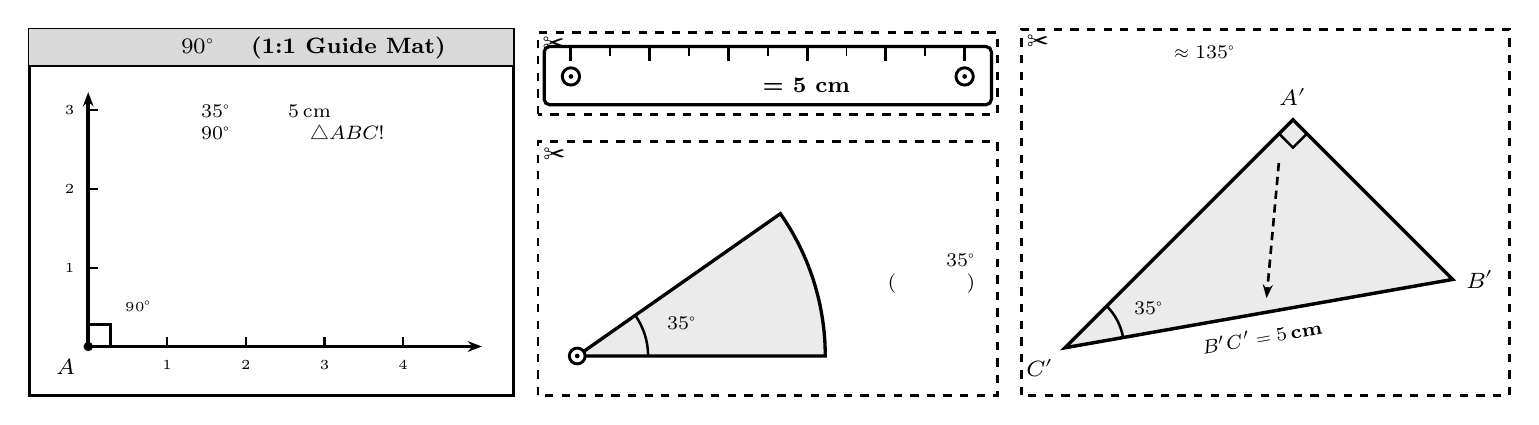
\begin{tikzpicture}[x=1cm, y=1cm, every node/.style={font=\scriptsize, text=black}]
  % === ឆ្វេង៖ ផ្ទាំងមុំកែង 90° គោល (6.15 cm x 4.65 cm) ===
  \begin{scope}[shift={(0,0)}]
    \draw[black, line width=1.1pt] (0,0) rectangle (6.15, 4.65);
    \fill[headgray] (0, 4.18) rectangle (6.15, 4.65);
    \draw[black, line width=0.9pt] (0, 4.18) -- (6.15, 4.18);
    \node[font=\footnotesize] at (3.08, 4.41) {\textbf{ផ្ទាំងមុំកែង $90^\circ$ គោល (\en{1:1 Guide Mat})}};
    % ជ្រុងកែង A=(0.75, 0.62)
    \coordinate (MA) at (0.75, 0.62);
    \coordinate (MX) at (5.75, 0.62);
    \coordinate (MY) at (0.75, 3.85);
    \draw[black, line width=1.35pt, -{Stealth[length=1.8mm]}] (MA) -- (MX);
    \draw[black, line width=1.35pt, -{Stealth[length=1.8mm]}] (MA) -- (MY);
    \foreach \kx in {1,2,3,4}{
      \draw[black, line width=0.85pt] ($(MA)+(\kx,0)$) -- ($(MA)+(\kx,0.12)$);
      \node[below=1.5pt, font=\tiny] at ($(MA)+(\kx,0)$) {\en{\kx}};
    }
    \foreach \ky in {1,2,3}{
      \draw[black, line width=0.85pt] ($(MA)+(0,\ky)$) -- ($(MA)+(0.12,\ky)$);
      \node[left=1.5pt, font=\tiny] at ($(MA)+(0,\ky)$) {\en{\ky}};
    }
    \pic[draw=black, line width=0.95pt, angle radius=2.8mm]{right angle=MX--MA--MY};
    \fill[black] (MA) circle (0.06);
    \node[below left=1pt, font=\footnotesize] at (MA) {$A$};
    \node[above right=1pt, font=\tiny] at ($(MA)+(0.32,0.28)$) {$90^\circ$};
    \node[anchor=north west, font=\scriptsize, align=left] at (1.35, 3.82) {ដាក់ស្នៀត $35^\circ$ និងបន្ទះ $5\unit{cm}$\\ទល់កាំកែង $90^\circ$ ដើម្បីចាក់សោ $\tri{ABC}$!};
  \end{scope}

  % === កណ្ដាល៖ បន្ទះអ៊ីប៉ូតេនុស 5.0 cm + ស្នៀតមុំ 35° (x=6.45 .. 12.35) ===
  % លើ៖ បន្ទះអ៊ីប៉ូតេនុស 5.0 cm (0..5 cm)
  \begin{scope}[shift={(6.88, 4.05)}]
    \draw[black, dashed, line width=0.95pt] (-0.42, -0.48) rectangle (5.42, 0.56);
    \node[anchor=north west, inner sep=1pt, font=\footnotesize] at (-0.40, 0.54) {\scissors};
    \draw[black, line width=1.15pt, rounded corners=2pt, fill=white] (-0.34, -0.36) rectangle (5.34, 0.38);
    \foreach \h in {0,0.5,...,5.0}{\draw[black, line width=0.65pt] (\h, 0.38) -- (\h, 0.26);}
    \foreach \k in {0,...,5}{\draw[black, line width=1.05pt] (\k, 0.38) -- (\k, 0.19);}
    \draw[black, line width=1.05pt, fill=white] (0,0) circle (0.11); \fill[black] (0,0) circle (0.03);
    \draw[black, line width=1.05pt, fill=white] (5,0) circle (0.11); \fill[black] (5,0) circle (0.03);
    \node[font=\footnotesize] at (2.5, -0.11) {\textbf{អ៊ីប៉ូតេនុស \en{= 5 cm}}};
  \end{scope}

  % ក្រោម៖ ស្នៀតមុំស្រួច 35° (កាត់) - r=3.15cm leaving wide clean right zone for label
  \begin{scope}[shift={(6.46, 0)}]
    \draw[black, dashed, line width=0.95pt] (0, 0) rectangle (5.84, 3.22);
    \node[anchor=north west, inner sep=1pt, font=\footnotesize] at (0.03, 3.19) {\scissors};
    \coordinate (W0) at (0.50, 0.50);
    \coordinate (W1) at (3.65, 0.50);
    \coordinate (W2) at ($(W0)+(35:3.15)$);
    \fill[panelgray] (W0) -- (W1) arc (0:35:3.15) -- cycle;
    \draw[black, line width=1.2pt] (W0) -- (W1) arc (0:35:3.15) -- cycle;
    \pic[draw=black, line width=0.9pt, angle radius=9.0mm]{angle=W1--W0--W2};
    \node[font=\scriptsize] at ($(W0)+(17.5:1.40)$) {\textbf{$35^\circ$}};
    \draw[black, line width=1.05pt, fill=white] (W0) circle (0.10); \fill[black] (W0) circle (0.03);
    \node[anchor=east, font=\scriptsize, align=right] at (5.68, 1.55) {\textbf{ស្នៀតមុំ $35^\circ$}\\(កាត់ដាក់ផ្ទៀង)};
  \end{scope}

  % === ស្ដាំ៖ ត្រីកោណកែងតេស្តបង្វិល ~135° (A'B'C': B'C'=5.00 cm, ∠A'=90°, ∠C'=35°) ===
  \begin{scope}[shift={(12.60, 0)}]
    \draw[black, dashed, line width=0.95pt] (0, 0) rectangle (6.20, 4.65);
    \node[anchor=north west, inner sep=1pt, font=\footnotesize] at (0.03, 4.62) {\scissors};
    \node[anchor=north west, font=\scriptsize] at (0.48, 4.56) {\textbf{ត្រីកោណតេស្តបង្វិល $\approx 135^\circ$}};
    % Exact 1:1 135 deg rotated coordinates shifted well inside box:
    \coordinate (Ap) at (3.45, 3.50);
    \coordinate (Cp) at (0.5538, 0.6038);
    \coordinate (Bp) at (5.4779, 1.4721);
    \fill[panelgray] (Ap) -- (Bp) -- (Cp) -- cycle;
    \draw[black, line width=1.25pt] (Ap) -- (Bp) -- (Cp) -- cycle;
    \pic[draw=black, line width=0.9pt, angle radius=2.5mm]{right angle=Cp--Ap--Bp};
    \pic[draw=black, line width=0.9pt, angle radius=7.5mm]{angle=Bp--Cp--Ap};
    \node[font=\scriptsize] at ($(Cp)+(25:1.18)$) {$35^\circ$};
    \draw[hypArrow] ($(Ap)+(-0.18,-0.55)$) -- ($(Bp)!0.48!(Cp)+(0,0.18)$);
    \node[below=2pt, rotate=10, font=\scriptsize] at ($(Bp)!0.50!(Cp)$) {\textbf{$B'C' = 5\unit{cm}$}};
    \node[above=1.5pt, font=\footnotesize] at (Ap) {$A'$};
    \node[right=1.5pt, font=\footnotesize] at (Bp) {$B'$};
    \node[below left=0.5pt, font=\footnotesize] at (Cp) {$C'$};
  \end{scope}
\end{tikzpicture}
\end{center}

\vspace{4pt}

% --- ផ្នែកទី ២៖ POE 2A (អ៊ីប៉ូតេនុស 5 cm vs ជ្រុងកែង 5 cm → អ៊ីប៉ូតេនុស ≈ 6.1 cm) ---
\textbf{២. សកម្មភាព \en{2A} (\en{POE 2A}) ៖ អន្ទាក់អ៊ីប៉ូតេនុស $5\unit{cm}$ ទល់ជ្រុងកែង $5\unit{cm}$ (ខ្នាតពិត \en{x=1cm, y=1cm})}

\vspace{2pt}
\noindent
\begin{minipage}[c]{11.55cm}
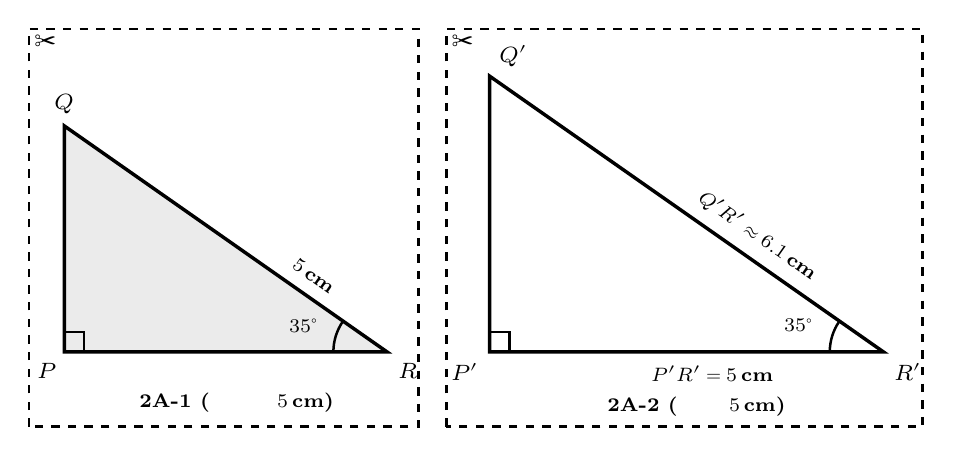
\begin{tikzpicture}[x=1cm, y=1cm, every node/.style={font=\scriptsize, text=black}]
  % === 2A-1: Hypotenuse QR = 5.0 cm, ∠P=90°, ∠R=35° (PR=4.0958, PQ=2.8679) ===
  \begin{scope}[shift={(0,0)}]
    \draw[black, dashed, line width=0.95pt] (0, 0) rectangle (4.95, 5.05);
    \node[anchor=north west, inner sep=1pt, font=\footnotesize] at (0.03, 5.02) {\scissors};
    \coordinate (P) at (0.45, 0.95);
    \coordinate (R) at (4.5458, 0.95);
    \coordinate (Q) at (0.45, 3.8179);
    \fill[panelgray] (P) -- (Q) -- (R) -- cycle;
    \draw[black, line width=1.25pt] (P) -- (Q) -- (R) -- cycle;
    \pic[draw=black, line width=0.9pt, angle radius=2.5mm]{right angle=R--P--Q};
    \pic[draw=black, line width=0.9pt, angle radius=6.8mm]{angle=Q--R--P};
    \node[font=\scriptsize] at ($(R)+(162.5:1.10)$) {$35^\circ$};
    \node[above right=1pt, rotate=-35, font=\scriptsize] at ($(Q)!0.48!(R)$) {\textbf{អ៊ីប៉ូតេនុស $5\unit{cm}$}};
    \node[below left=0.5pt, font=\footnotesize] at (P) {$P$};
    \node[above=1pt, font=\footnotesize] at (Q) {$Q$};
    \node[below right=0.5pt, font=\footnotesize] at (R) {$R$};
    \node[font=\scriptsize] at (2.48, 0.30) {\textbf{កាត \en{2A-1} (អ៊ីប៉ូតេនុស $5\unit{cm}$)}};
  \end{scope}

  % === 2A-2: Leg P'R' = 5.0 cm, ∠P'=90°, ∠R'=35° -> Hyp Q'R' = 6.104 cm ≈ 6.1 cm ===
  \begin{scope}[shift={(5.30, 0)}]
    \draw[black, dashed, line width=0.95pt] (0, 0) rectangle (6.05, 5.05);
    \node[anchor=north west, inner sep=1pt, font=\footnotesize] at (0.03, 5.02) {\scissors};
    \coordinate (Pp) at (0.55, 0.95);
    \coordinate (Rp) at (5.55, 0.95);
    \coordinate (Qp) at (0.55, 4.4510);
    \fill[white] (Pp) -- (Qp) -- (Rp) -- cycle;
    \draw[black, line width=1.25pt] (Pp) -- (Qp) -- (Rp) -- cycle;
    \pic[draw=black, line width=0.9pt, angle radius=2.5mm]{right angle=Rp--Pp--Qp};
    \pic[draw=black, line width=0.9pt, angle radius=6.8mm]{angle=Qp--Rp--Pp};
    \node[font=\scriptsize] at ($(Rp)+(162.5:1.12)$) {$35^\circ$};
    \node[above right=1pt, rotate=-35, font=\scriptsize] at ($(Qp)!0.48!(Rp)$) {\textbf{$Q'R' \approx 6.1\unit{cm}$}};
    \node[below=1.5pt, font=\scriptsize] at ($(Pp)!0.50!(Rp)$) {\textbf{ជ្រុងកែង $P'R' = 5\unit{cm}$}};
    \node[below left=0.5pt, font=\footnotesize] at (Pp) {$P'$};
    \node[above right=0pt, font=\footnotesize] at (Qp) {$Q'$};
    \node[below right=0.5pt, font=\footnotesize] at (Rp) {$R'$};
    \node[font=\scriptsize] at (3.02, 0.25) {\textbf{កាត \en{2A-2} (ជ្រុងកែង $5\unit{cm}$)}};
  \end{scope}
\end{tikzpicture}
\end{minipage}%
\hfill
\begin{minipage}[c]{7.15cm}
  \begin{tcolorbox}[
    enhanced, sharp corners, colback=white, colframe=black,
    boxrule=1.05pt, boxsep=1pt, top=4pt, bottom=4pt, left=5pt, right=5pt,
    title={\textbf{កំណត់ត្រា \en{POE 2A} ៖ អ៊ីប៉ូតេនុស \en{vs} ជ្រុងកែង}},
    colbacktitle=headgray, coltitle=black, fonttitle=\fontsize{8.4pt}{11.5pt}\selectfont
  ]
    \raggedright\fontsize{8.0pt}{11.7pt}\selectfont
    \textbf{\en{P} \en{--} ទស្សន៍ទាយ៖} មាន $90^\circ, 35^\circ$ និងជ្រុង $5\unit{cm}$ ដូចគ្នា តើត្រីកោណទាំងពីរប៉ុនគ្នាទេ?\\
    \chkbox\ ប៉ុនគ្នា \hspace{0.4cm} \chkbox\ មិនប្រាកដ\\[4pt]
    \textbf{\en{O} \en{--} សង្កេត (កាត់ផ្ទៀងត្រួត)៖}\\
    ដាក់ $\tri{PQR}$ លើ $\tri{P'Q'R'}$ ឃើញអ៊ីប៉ូតេនុស $Q'R' \approx 6.1\unit{cm} \neq 5\unit{cm}$៖\\
    \chkbox\ ត្រួតបេះបិទ \hspace{0.2cm} \chkbox\ ខុសទំហំ ($\ncg$)\\[4pt]
    \textbf{\en{E} \en{--} ពន្យល់៖} ហេតុអ្វីត្រូវប្រើ \textbf{អ៊ីប៉ូតេនុស} (ឈម $90^\circ$) ស្មើគ្នា?\\[3pt]
    \rule{\linewidth}{0.55pt}\\[10pt]
    \rule{\linewidth}{0.55pt}
  \end{tcolorbox}
\end{minipage}

\vspace{4pt}

% --- ផ្នែកទី ៣៖ POE 2B (ផ្ទាំងបត់ក្រដាសកន្លះបន្ទាត់ពុះមុំ ∠XOY — MA ⊥ OX, MB ⊥ OY vs ទ្រេត MD មិនកែង OY) ---
\textbf{៣. សកម្មភាព \en{2B} (\en{POE 2B}) ៖ ផ្ទាំងបត់កន្លះបន្ទាត់ពុះមុំ $\ang{XOY}$ និងចម្ងាយកែង vs ចម្ងាយទ្រេត (ខ្នាតពិត \en{x=1cm, y=1cm})}

\vspace{2pt}
\noindent
\begin{minipage}[c]{9.05cm}
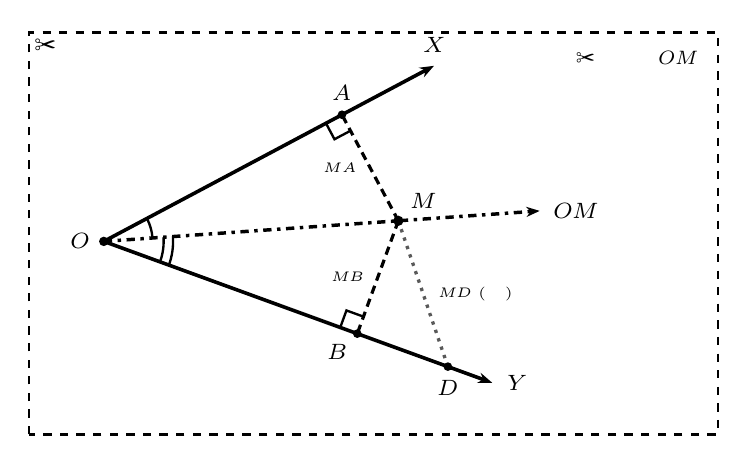
\begin{tikzpicture}[x=1cm, y=1cm, every node/.style={font=\scriptsize, text=black}]
  \draw[black, dashed, line width=0.95pt] (0, 0) rectangle (8.75, 5.10);
  \node[anchor=north west, inner sep=1pt, font=\footnotesize] at (0.03, 5.07) {\scissors};
  \node[anchor=north east, font=\scriptsize] at (8.60, 5.00) {កាត់ \scissors{} រួចបត់តាម $OM$};
  % O=(0.95, 2.45), OM at +4 deg, OX at +28 deg, OY at -20 deg (bisected!)
  \coordinate (O) at (0.95, 2.45);
  \coordinate (X) at ($(O)+(28:4.75)$);
  \coordinate (Y) at ($(O)+(-20:5.25)$);
  \coordinate (M) at ($(O)+(4:3.75)$);
  \coordinate (Mold) at ($(O)+(4:5.55)$);
  % Perpendicular drops: OA = OB = 3.75 * cos(24) = 3.4258 cm
  \coordinate (A) at ($(O)+(28:3.4258)$);
  \coordinate (B) at ($(O)+(-20:3.4258)$);
  % Slanted decoy D on OY at 4.65 cm
  \coordinate (D) at ($(O)+(-20:4.65)$);

  \draw[black, line width=1.3pt, -{Stealth[length=1.8mm]}] (O) -- (X) node[above=1pt, font=\footnotesize] {$X$};
  \draw[black, line width=1.3pt, -{Stealth[length=1.8mm]}] (O) -- (Y) node[right=1.5pt, font=\footnotesize] {$Y$};
  \draw[black, line width=1.25pt, dash dot, -{Stealth[length=1.7mm]}] (O) -- (Mold) node[right=1pt, font=\footnotesize] {$OM$};
  \node[above=2pt, rotate=4, font=\tiny] at ($(O)+(4:1.90)$) {\textbf{បន្ទាត់បត់ពុះមុំ}};

  \draw[black, densely dashed, line width=1.15pt] (M) -- (A) node[midway, left=1pt, font=\tiny] {$MA$};
  \draw[black, densely dashed, line width=1.15pt] (M) -- (B) node[midway, left=1pt, font=\tiny] {$MB$};
  \pic[draw=black, line width=0.85pt, angle radius=2.3mm]{right angle=O--A--M};
  \pic[draw=black, line width=0.85pt, angle radius=2.3mm]{right angle=O--B--M};

  \draw[darkline, dotted, line width=1.2pt] (M) -- (D) node[midway, right=1.5pt, font=\tiny] {$MD$ (ទ្រេត)};

  \pic[draw=black, line width=0.85pt, angle radius=6.2mm]{angle=M--O--X};
  \pic[draw=black, line width=0.85pt, angle radius=7.6mm]{angle=Y--O--M};
  \pic[draw=black, line width=0.85pt, angle radius=8.8mm]{angle=Y--O--M};

  \fill[black] (O) circle (0.06) node[left=1.5pt, font=\footnotesize] {$O$};
  \fill[black] (M) circle (0.065) node[above right=1pt, font=\footnotesize] {$M$};
  \fill[black] (A) circle (0.055) node[above=1.5pt, font=\footnotesize] {$A$};
  \fill[black] (B) circle (0.055) node[below left=0.5pt, font=\footnotesize] {$B$};
  \fill[black] (D) circle (0.055) node[below=1.5pt, font=\footnotesize] {$D$};
\end{tikzpicture}
\end{minipage}%
\hfill
\begin{minipage}[c]{9.65cm}
  \begin{tcolorbox}[
    enhanced, sharp corners, colback=white, colframe=black,
    boxrule=1.05pt, boxsep=1pt, top=5pt, bottom=5pt, left=6pt, right=6pt,
    title={\textbf{កំណត់ត្រា \en{POE 2B} ៖ បត់កន្លះពុះមុំ $\ang{XOY}$ \& ចម្ងាយកែង}},
    colbacktitle=headgray, coltitle=black, fonttitle=\fontsize{8.5pt}{11.5pt}\selectfont
  ]
    \raggedright\fontsize{8.2pt}{12.1pt}\selectfont
    \textbf{\en{P} \en{--} ទស្សន៍ទាយ៖} ពេលបត់ក្រដាសតាម $OM$ ឱ្យ $OX$ ត្រួតលើ $OY$ តើអង្កត់ណាពី $M$ ដែលមានប្រវែងស្មើគ្នា ($MA$ ទល់ $MB$ ឬ $MD$)?\\
    \chkbox\ $MA = MB$ \hspace{0.3cm} \chkbox\ $MA = MD$ \hspace{0.3cm} \chkbox\ មិនស្មើទេ\\[5pt]
    \textbf{\en{O} \en{--} សង្កេត (បត់ក្រដាស \& វាស់ខ្នាត ១:១)៖}\\
    $\bullet$ ចំណុច $A$ ត្រួតបេះបិទលើ $\underline{\hspace{0.8cm}}$ ($\ang{A}=\ang{B}=90^\circ$) $\Rightarrow MA = MB \approx 1.5\unit{cm}$។\\
    $\bullet$ អង្កត់ទ្រេត $MD$ (មិនកែង $OY$) មានប្រវែង $\approx 2.0\unit{cm}$ ($\underline{\hspace{1.4cm}}$ ជាង $MA$)។\\[5pt]
    \textbf{\en{E} \en{--} ពន្យល់ (សរុប \en{E2})៖} ១) ត្រីកោណកែងត្រូវមាន \textbf{អ៊ីប៉ូតេនុស} និង \textbf{មុំស្រួច} ស្មើគ្នា; ២) ចម្ងាយពី $M$ ទៅជ្រុងមុំត្រូវវាស់តាមអង្កត់ \textbf{កែង $90^\circ$}៖\\[3pt]
    \rule{\linewidth}{0.55pt}
  \end{tcolorbox}
\end{minipage}

\clearpage

% ============================================================================
% ទំព័រទី ២៖ E4 Elaborate — កាតព្រួញឈម 90° និងអ៊ីប៉ូតេនុសរួម OM (២ ប័ណ្ណ)
% ============================================================================
\pagebanner{សម្ភារៈទី ២៖ កាតព្រួញឈម \enbf{90}$^\circ$ និងអ៊ីប៉ូតេនុសរួម \enbf{OM}}{ទំព័រ ២/៦ \en{-- E4 Elaborate} (កាត់ ២ ប័ណ្ណ \scissors)}

\newcommand{\eFourCardHA}[1]{%
\begin{tcolorbox}[
  enhanced, sharp corners, colback=white, colframe=white,
  borderline={1.0pt}{0pt}{black, dashed},
  boxsep=1pt, top=4pt, bottom=4pt, left=5pt, right=5pt
]
  \begin{tcolorbox}[
    enhanced, sharp corners, colback=headgray, colframe=black,
    boxrule=0.8pt, boxsep=1pt, top=2.5pt, bottom=2.5pt, left=5pt, right=5pt, after skip=5pt
  ]
    \fontsize{8.5pt}{11.5pt}\selectfont
    \textbf{\scissors\ កាតសកម្មភាព \en{E4} (#1) \en{--} កាតព្រួញឈម $90^\circ$ និងអ៊ីប៉ូតេនុសរួម $OM$} \hfill ក្រុម៖ $\underline{\hspace{2.8cm}}$
  \end{tcolorbox}

  \noindent
  \begin{minipage}[t]{7.55cm}
    \vspace{0pt}
    \fontsize{8.2pt}{11.6pt}\selectfont
    \textbf{លំហាត់គំរូ (ទំព័រ ១៥៣)៖} គេឱ្យ $M$ ជាចំណុចមួយស្ថិតនៅលើកន្លះបន្ទាត់ពុះនៃ $\ang{XOY}$~។ តាម $M$ គូសបន្ទាត់កែងនឹង $OX$ ត្រង់ $A$ និង $OY$ ត្រង់ $B$~។ បង្ហាញថា $MA = MB$~។
    \begin{center}
    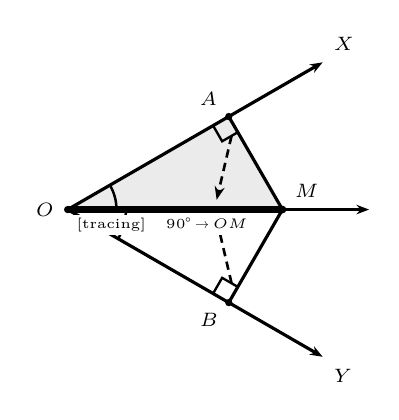
\begin{tikzpicture}[scale=0.88, every node/.style={font=\scriptsize, text=black}]
      % Exact Book p. 153 WITHOUT "/" ticks on OA, OB!
      \coordinate (O) at (0,0);
      \coordinate (X) at (30:4.25);
      \coordinate (Y) at (-30:4.25);
      \coordinate (M) at (0:3.10);
      \coordinate (Mend) at (0:4.35);
      % Exact perp feet: OA = OB = 3.10*cos(30) = 2.6847
      \coordinate (A) at (30:2.6847);
      \coordinate (B) at (-30:2.6847);

      \fill[panelgray] (O) -- (A) -- (M) -- cycle;
      \draw[black, line width=1.15pt, -{Stealth[length=1.6mm]}] (O) -- (X) node[above right=0.5pt] {$X$};
      \draw[black, line width=1.15pt, -{Stealth[length=1.6mm]}] (O) -- (Y) node[below right=0.5pt] {$Y$};
      \draw[black, line width=1.15pt] (A) -- (M) -- (B);
      % Common hypotenuse OM emphasized + [tracing]
      \draw[black, line width=2.3pt] (O) -- (M);
      \draw[black, line width=1.0pt, -{Stealth[length=1.6mm]}] (M) -- (Mend);

      % 90° boxes at A and B
      \pic[draw=black, line width=0.85pt, angle radius=2.3mm]{right angle=O--A--M};
      \pic[draw=black, line width=0.85pt, angle radius=2.3mm]{right angle=O--B--M};
      % Equal angle arcs at O (ONLY arcs, ZERO "/" on OA, OB!)
      \pic[draw=black, line width=0.9pt, angle radius=6.2mm]{angle=M--O--X};
      \pic[draw=black, line width=0.9pt, angle radius=7.4mm]{angle=Y--O--M};

      % Dashed [tracing] arrows 90° -> OM positioned cleanly on right so label has zero touch
      \draw[hypArrow] ($(A)+(0.04,-0.28)$) -- (2.15, 0.14);
      \draw[hypArrow] ($(B)+(0.04,0.28)$) -- (2.15, -0.14);
      \node[font=\tiny, fill=white, inner sep=1pt] at (1.35, -0.22) {\en{[tracing]} ឈម $90^\circ \to OM$};

      \fill[black] (O) circle (1.5pt) node[left=1.5pt] {$O$};
      \fill[black] (A) circle (1.5pt) node[above left=0.5pt] {$A$};
      \fill[black] (B) circle (1.5pt) node[below left=0.5pt] {$B$};
      \fill[black] (M) circle (1.6pt) node[above right=1pt] {$M$};
    \end{tikzpicture}
    \end{center}
    \begin{tcolorbox}[enhanced, sharp corners, colback=panelgray, colframe=black, boxrule=0.7pt, boxsep=1pt, top=2.5pt, bottom=2.5pt, left=4pt, right=4pt]
      \fontsize{7.55pt}{10.8pt}\selectfont
      \textbf{ពិនិត្យក្រោយ (\en{EIA} ៣០ វិនាទី)៖} បើរំកិល $M$ តាមកន្លះបន្ទាត់ពុះ $OM$ (រក្សា $MA\perp OX, MB\perp OY$) តើ $MA=MB$ នៅពិតទេ? \chkbox\ ពិតជានិច្ច \chkbox\ ប្រែប្រួល\\
      ហេតុអ្វី\textbf{ហាមគូស} \tickone\ លើ $OA, OB$ មុនស្រាយ? ($\underline{\hspace{2.1cm}}$)
    \end{tcolorbox}
  \end{minipage}\hfill
  \begin{minipage}[t]{10.25cm}
    \vspace{0pt}
    \begin{tcolorbox}[enhanced, sharp corners, colback=panelgray, colframe=black, boxrule=0.8pt, boxsep=1pt, top=3.5pt, bottom=3.5pt, left=5pt, right=5pt]
      \raggedright\fontsize{8.05pt}{12.0pt}\selectfont
      \textbf{ជំហាន ១ [ចង្អុល \en{[tracing]} ប្រអប់ $90^\circ \rightarrow OM$ រួម]៖}\\
      \chkbox\ គូសប្រអប់ $90^\circ$ ត្រង់ $A, B$ (\cnum{1}) \hspace{0.15cm}
      \chkbox\ គូសធ្នូមុំស្មើត្រង់ $O$ (\cnum{2})\\
      \chkbox\ អូសម្រាមដៃ \en{[tracing]} ពី $90^\circ$ ទៅ $OM$ (អ៊ីប៉ូតេនុសរួម \cnum{3}) \hspace{0.1cm} (\textbf{គ្មាន \tickone\ លើ $OA, OB$!})\\[4pt]
      \textbf{ជំហាន ២ [កែទំ.១៥៣ \& ស្រាយ ៣ លក្ខខណ្ឌ \cnum{1}--\cnum{3}]៖}\\
      ក្នុងត្រីកោណកែង $OMA$ និងត្រីកោណកែង $\underline{\hspace{0.85cm}}$ \textit{(កែមិនមែន $OMA$ ទេ!)} មាន៖\\
      \en{1)} $\ang{OAM} = \ang{\underline{\hspace{0.85cm}}} = 90^\circ$ \hspace{0.2cm} (\cnum{1} $\underline{\hspace{1.8cm}}$)\\
      \en{2)} $\ang{MOA} = \ang{\underline{\hspace{0.85cm}}}$ \hspace{0.2cm} (\cnum{2} $OM$ ពុះ $\ang{XOY}$)\\
      \en{3)} $OM = \underline{\hspace{0.85cm}}$ \hspace{0.2cm} (\cnum{3} អ៊ីប៉ូតេនុសរួម ឈម $90^\circ$)\\[4pt]
      \textbf{ជំហាន ៣ [សន្និដ្ឋាន អ.ម \cnum{4} \& វិបាកចម្ងាយកែង \cnum{5}]៖}\\
      ដូចនេះ $\tri{OMA}\;\underline{\hspace{0.45cm}}\;\tri{\underline{\hspace{0.85cm}}}$ \hspace{0.2cm} (\cnum{4} $\underline{\hspace{1.65cm}}$)\\
      \textbf{វិបាក (\cnum{5})៖} $MA = \underline{\hspace{0.75cm}}$ (ចម្ងាយកែងពី $M$ ទៅ $OX, OY$ ស្មើគ្នា!)
    \end{tcolorbox}
    \vspace{3pt}
    {\fontsize{7.2pt}{10.1pt}\selectfont
    \textbf{ធនាគារអំណះអំណាង៖} \cnum{1} បម្រាប់/មុំកែង $90^\circ$ \en{|} \cnum{2} មុំស្រួចស្មើ (ពុះមុំ/$90^\circ-\text{មុំ}$) \en{|} \cnum{3} អ៊ីប៉ូតេនុសស្មើ/រួម \en{|} \cnum{4} អ.ម (\en{HA}) \en{|} \cnum{5} ធាតុត្រូវគ្នា/ចម្ងាយកែងស្មើ}
  \end{minipage}
\end{tcolorbox}%
}

\eFourCardHA{ប័ណ្ណទី ១}

\vspace{7pt}
\noindent\scissors\ \dotfill\ \textbf{កាត់តាមស្នាមចុចចែកជា ២ ប័ណ្ណ (\en{Cut Along Dashed Line})} \dotfill\ \scissors
\vspace{7pt}

\eFourCardHA{ប័ណ្ណទី ២}

\clearpage

% ============================================================================
% ទំព័រទី ៣៖ E5 Evaluate — ស្ទូឌីយោផ្ទៀងកម្ពស់ខ្វែង ៣ តួនាទី (២ សន្លឹក)
% ============================================================================
\pagebanner{សម្ភារៈទី ៣៖ ស្ទូឌីយោផ្ទៀងកម្ពស់ខ្វែង ៣ តួនាទី \enbf{(E5 \& E1)}}{ទំព័រ ៣/៦ \en{-- E5 Evaluate} (កាត់ ២ សន្លឹក \scissors)}

\newcommand{\eFiveSheetHA}[1]{%
\begin{tcolorbox}[
  enhanced, sharp corners, colback=white, colframe=white,
  borderline={1.0pt}{0pt}{black, dashed},
  boxsep=1pt, top=3pt, bottom=3pt, left=4.5pt, right=4.5pt
]
  \begin{tcolorbox}[
    enhanced, sharp corners, colback=headgray, colframe=black,
    boxrule=0.8pt, boxsep=1pt, top=2pt, bottom=2pt, left=5pt, right=5pt, after skip=3.5pt
  ]
    \fontsize{7.85pt}{10.8pt}\selectfont
    \textbf{\scissors\ ស្ទូឌីយោផ្ទៀងកម្ពស់ខ្វែង (#1) \en{--} ក្រុម៖} $\underline{\hspace{1.8cm}}$ \hfill \textbf{ប្រតិបត្តិ (ទំ.១៥៤)៖} $\tri{ABC}$ សមបាទ ($AB=AC$), $BD\perp AC, CE\perp AB \Rightarrow BD=CE,\; BE=CD$
  \end{tcolorbox}

  \renewcommand{\arraystretch}{1.04}
  \begin{tabular}{|L{6.15cm}|L{5.65cm}|L{5.30cm}|}
    \hline
    \cellcolor{panelgray}\centering\arraybackslash\fontsize{7.6pt}{10.2pt}\selectfont\textbf{តួនាទី ១៖ គូសសញ្ញា \en{\&} បំបែកត្រីកោណ}\newline {\fontsize{7.0pt}{9.2pt}\selectfont \textbf{\en{Pause-Ask!}} \en{--} ព្រួញ $90^\circ \to \text{Hyp}$} &
    \cellcolor{panelgray}\centering\arraybackslash\fontsize{7.6pt}{10.2pt}\selectfont\textbf{តួនាទី ២៖ សម្រាយ ៣ បន្ទាត់ \& \cnum{1}--\cnum{4}}\newline {\fontsize{7.0pt}{9.2pt}\selectfont សរសេរលក្ខខណ្ឌ \textbf{អ.ម (\en{HA})} ភ្ជាប់លេខ} &
    \cellcolor{panelgray}\centering\arraybackslash\fontsize{7.6pt}{10.2pt}\selectfont\textbf{តួនាទី ៣៖ វិបាក \cnum{5} \& បិទ \en{E1}}\newline {\fontsize{7.0pt}{9.2pt}\selectfont \textbf{\en{Pause-Review!}} ដកអង្កត់ \en{+} ជម្រាល/ទ្វារទឹក} \\ \hline

    % --- Column 1: Main Triangle ABC + Exploded ADB & AEC silhouettes ---
    {\centering
    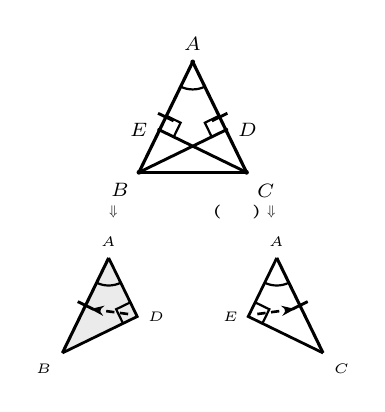
\begin{tikzpicture}[scale=0.61, every node/.style={font=\scriptsize, text=black}]
      % Main isosceles ∆ABC: A=(0,2.30), B=(-1.12,0), C=(1.12,0)
      % Exact altitude feet: D=(0.6906, 0.8817), E=(-0.6906, 0.8817)
      \coordinate (A) at (0, 2.30);
      \coordinate (B) at (-1.12, 0);
      \coordinate (C) at (1.12, 0);
      \coordinate (D) at (0.6906, 0.8817);
      \coordinate (E) at (-0.6906, 0.8817);
      \draw[black, line width=1.15pt, tk1] (A) -- (B);
      \draw[black, line width=1.15pt, tk1] (A) -- (C);
      \draw[black, line width=1.1pt] (B) -- (C);
      \draw[black, line width=1.05pt] (B) -- (D);
      \draw[black, line width=1.05pt] (C) -- (E);
      \pic[draw=black, line width=0.8pt, angle radius=2.0mm]{right angle=A--D--B};
      \pic[draw=black, line width=0.8pt, angle radius=2.0mm]{right angle=A--E--C};
      \pic[draw=black, line width=0.8pt, angle radius=3.5mm]{angle=B--A--C};
      \fill[black] (A) circle (1.4pt) node[above=0.5pt] {$A$};
      \fill[black] (B) circle (1.4pt) node[below left=0.5pt] {$B$};
      \fill[black] (C) circle (1.4pt) node[below right=0.5pt] {$C$};
      \fill[black] (D) circle (1.4pt) node[right=1pt] {$D$};
      \fill[black] (E) circle (1.4pt) node[left=1pt] {$E$};

      % បំបែកត្រីកោណត្រួតគ្នា (spaced well clear of B,C and lower A)
      \node[font=\tiny] at (0, -0.82) {$\Downarrow$ \textbf{បំបែកត្រីកោណត្រួតគ្នា (ផ្ទៀងងាយ)} $\Downarrow$};
      % Exploded ∆ADB
      \begin{scope}[shift={(-1.75, -3.76)}, scale=0.86]
        \coordinate (A1) at (0, 2.30); \coordinate (B1) at (-1.12, 0); \coordinate (D1) at (0.6906, 0.8817);
        \fill[panelgray] (A1) -- (B1) -- (D1) -- cycle;
        \draw[black, line width=1.1pt, tk1] (A1) -- (B1);
        \draw[black, line width=1.0pt] (A1) -- (D1) -- (B1);
        \pic[draw=black, line width=0.8pt, angle radius=2.0mm]{right angle=A1--D1--B1};
        \pic[draw=black, line width=0.8pt, angle radius=3.5mm]{angle=B1--A1--D1};
        \draw[hypArrow] ($(D1)+(-0.22,0.06)$) -- ($(A1)!0.52!(B1)+(0.14,-0.04)$);
        \node[above=0.5pt, font=\tiny] at (A1) {$A$};
        \node[below left=0.5pt, font=\tiny] at (B1) {$B$};
        \node[right=0.5pt, font=\tiny] at (D1) {$D$};
      \end{scope}
      % Exploded ∆AEC
      \begin{scope}[shift={(1.75, -3.76)}, scale=0.86]
        \coordinate (A2) at (0, 2.30); \coordinate (C2) at (1.12, 0); \coordinate (E2) at (-0.6906, 0.8817);
        \fill[white] (A2) -- (C2) -- (E2) -- cycle;
        \draw[black, line width=1.1pt, tk1] (A2) -- (C2);
        \draw[black, line width=1.0pt] (A2) -- (E2) -- (C2);
        \pic[draw=black, line width=0.8pt, angle radius=2.0mm]{right angle=A2--E2--C2};
        \pic[draw=black, line width=0.8pt, angle radius=3.5mm]{angle=E2--A2--C2};
        \draw[hypArrow] ($(E2)+(0.22,0.06)$) -- ($(A2)!0.52!(C2)+(-0.14,-0.04)$);
        \node[above=0.5pt, font=\tiny] at (A2) {$A$};
        \node[below right=0.5pt, font=\tiny] at (C2) {$C$};
        \node[left=0.5pt, font=\tiny] at (E2) {$E$};
      \end{scope}
    \end{tikzpicture}\par}
    \fontsize{7.1pt}{9.8pt}\selectfont
    \chkbox\ គូស $90^\circ$ ត្រង់ $D, E$, \tickone\ លើ $AB=AC$ និងព្រួញ $90^\circ \to AB, AC$\\
    \chkbox\ \textbf{\en{Pause-Ask!}} «ហេតុអ្វី $AB, AC$ ជាអ៊ីប៉ូតេនុស និងមុំ $\ang{A}$ រួម?»
    &
    % --- Column 2: Proof ①–④ ---
    \fontsize{7.55pt}{11.2pt}\selectfont
    ក្នុង $\tri{ADB}$ និង $\tri{AEC}$ មាន៖\par\vspace{2.5pt}
    \en{1)} $\ang{ADB} = \ang{\underline{\hspace{0.75cm}}} = 90^\circ$ (\cnum{1} $\underline{\hspace{1.15cm}}$)\par\vspace{2.5pt}
    \en{2)} $\ang{\underline{\hspace{0.45cm}}}$ ជាមុំស្រួចរួម (\cnum{2} $\underline{\hspace{1.35cm}}$)\par\vspace{2.5pt}
    \en{3)} អ៊ីប៉ូតេនុស $AB = \underline{\hspace{0.75cm}}$ (\cnum{3} ឈម $90^\circ$)\par\vspace{3pt}
    ដូចនេះ $\tri{ADB} \cg \tri{\underline{\hspace{0.75cm}}}$ (\cnum{4} $\underline{\hspace{1.15cm}}$)\par\vspace{5pt}
    \begin{tcolorbox}[enhanced, sharp corners, colback=panelgray, colframe=black, boxrule=0.6pt, boxsep=1pt, top=2.5pt, bottom=2.5pt, left=4pt, right=4pt]
      \raggedright\fontsize{6.8pt}{9.6pt}\selectfont
      \textbf{វិធីទី ២ (ចំណាំ)៖} ក៏អាចប្រើ $\tri{BDC}\cg\tri{CEB}$ (\cnum{4} អ.ម) ដោយអ៊ីប៉ូតេនុសរួម $BC=CB$ និង $\ang{B}=\ang{C}$!\\[2pt]
      \textbf{ធនាគារ៖} \cnum{1} មុំកែង $90^\circ$ \en{|} \cnum{2} មុំស្រួចស្មើ \en{|} \cnum{3} អ៊ីប៉ូតេនុស \en{|} \cnum{4} អ.ម
    \end{tcolorbox}
    &
    % --- Column 3: Pause-Review, BD=CE, BE=CD & E1 Closure ---
    \fontsize{7.45pt}{11.0pt}\selectfont
    \chkbox\ \textbf{\en{Pause-Review!}} ផ្ទៀងលំដាប់កំពូល៖\newline
    $A\leftrightarrow A,\; D\leftrightarrow\underline{\hspace{0.35cm}}\; (90^\circ),\; B\leftrightarrow\underline{\hspace{0.35cm}}$\par\vspace{2.5pt}
    \textbf{វិបាក (\cnum{5})៖} $BD = \underline{\hspace{0.65cm}}$ និង $AD = \underline{\hspace{0.65cm}}$\par\vspace{2.5pt}
    \textbf{ដកអង្កត់៖}\newline
    $BE = AB - \underline{\hspace{0.55cm}} = AC - \underline{\hspace{0.55cm}} = \underline{\hspace{0.55cm}}$ (\cnum{5})\par\vspace{4pt}
    \begin{tcolorbox}[enhanced, sharp corners, colback=panelgray, colframe=black, boxrule=0.7pt, boxsep=1pt, top=2.5pt, bottom=2.5pt, left=4pt, right=4pt]
      \raggedright\fontsize{6.95pt}{9.8pt}\selectfont
      \textbf{បិទបេសកកម្ម \en{E1} (ជម្រាល \& ទ្វារទឹក)៖}\\
      $\bullet$ ជម្រាល $5\unit{m}$ ($30^\circ$) $\Rightarrow$ កែងស្មើដោយ \cnum{4} $\underline{\hspace{0.55cm}}$!\\
      $\bullet$ ទ្វារទឹក $M$ លើពុះមុំ $OM$, $MA\perp OX, MB\perp OY \Rightarrow MA=MB$ (\cnum{5})!
    \end{tcolorbox}
    \\[1pt] \hline
  \end{tabular}
\end{tcolorbox}%
}

\eFiveSheetHA{សន្លឹកទី ១}

\vspace{5pt}
\noindent\scissors\ \dotfill\ \textbf{កាត់តាមស្នាមចុចចែកជា ២ សន្លឹក (\en{Cut Along Dashed Line})} \dotfill\ \scissors
\vspace{5pt}

\eFiveSheetHA{សន្លឹកទី ២}

\clearpage

% ============================================================================
% ទំព័រទី ៤៖ ផ្ទាំងយោងប្រចាំថ្នាក់រៀន — ទ្រឹស្ដីបទ អ.ម (HA), ពុះមុំ & ធនាគារ ①–⑤
% ============================================================================
\begin{tcolorbox}[
  enhanced, sharp corners, colback=white, colframe=black,
  boxrule=1.5pt, borderline={0.6pt}{2.2pt}{black},
  boxsep=1pt, top=4pt, bottom=4pt, left=6pt, right=6pt
]
  \begin{center}
    {\muol\fontsize{11.4pt}{16pt}\selectfont ទ្រឹស្ដីបទ អ\enbf{.}ម \enbf{(HA) ,} លក្ខណៈពុះមុំ និងធនាគារ \cnum{1}\en{--}\cnum{5}}\\[1pt]
    {\fontsize{8.6pt}{12.0pt}\selectfont ផ្ទាំងយោងប្រចាំថ្នាក់រៀន (ស-ខ្មៅ) \en{--} មេរៀនទី១២ (១.៣.១) អ៊ីប៉ូតេនុសប៉ុនគ្នា និងមុំស្រួចមួយប៉ុនគ្នា}\\[2pt]
    \khmflourish
  \end{center}
  \vspace{1pt}

  % --- ផ្នែកទី ១៖ ទ្រឹស្ដីបទ អ.ម + រូបបង្វិល ~135° & ក្បួនប្រអប់កែង 90° -> ព្រួញអ៊ីប៉ូតេនុស ---
  \noindent
  \begin{minipage}[c]{9.0cm}
    \begin{tcolorbox}[enhanced, sharp corners, colback=panelgray, colframe=black, boxrule=0.85pt, boxsep=1pt, top=3pt, bottom=3pt, left=5pt, right=5pt]
      \raggedright\fontsize{8.0pt}{11.4pt}\selectfont
      \textbf{ទ្រឹស្ដីបទ (អ.ម / \en{HA})៖} ត្រីកោណកែងពីរប៉ុនគ្នាកាលណាវាមាន \textbf{អ៊ីប៉ូតេនុសប៉ុនគ្នា} និង \textbf{មុំស្រួចមួយប៉ុនគ្នា}~។\\[2.5pt]
      \textbf{ក្បួន «ប្រអប់កែង $90^\circ \rightarrow$ ព្រួញចង្អុលអ៊ីប៉ូតេនុស»៖} ទោះត្រីកោណបង្វិល $\approx 135^\circ$ ក៏ត្រូវចាប់ផ្ដើមគូសព្រួញពីប្រអប់ $90^\circ$ ទៅរកជ្រុងឈម (\textbf{អ៊ីប៉ូតេនុស}) មុនជានិច្ច!
    \end{tcolorbox}
  \end{minipage}\hfill
  \begin{minipage}[c]{8.8cm}
    \centering
    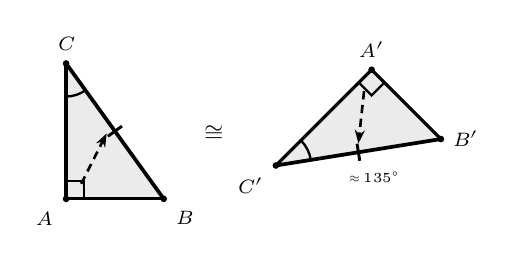
\begin{tikzpicture}[scale=0.80, every node/.style={font=\scriptsize, text=black}]
      % ត្រីកោណទី១ (Upright)
      \coordinate (A) at (0,0);
      \coordinate (B) at (1.55,0);
      \coordinate (C) at (0, 2.15);
      \fill[panelgray] (A) -- (B) -- (C) -- cycle;
      \draw[black, line width=1.15pt] (C) -- (A) -- (B);
      \draw[black, line width=1.35pt, tk1] (B) -- (C);
      \pic[draw=black, line width=0.85pt, angle radius=2.3mm]{right angle=B--A--C};
      \pic[draw=black, line width=0.85pt, angle radius=4.2mm]{angle=A--C--B};
      \draw[hypArrow] ($(A)+(0.24,0.24)$) -- ($(B)!0.52!(C)+(-0.10,-0.08)$);
      \fill[black] (A) circle (1.5pt) (B) circle (1.5pt) (C) circle (1.5pt);
      \node[below left=1pt] at (A) {$A$};
      \node[below right=1pt] at (B) {$B$};
      \node[above=1pt] at (C) {$C$};

      \node[font=\small] at (2.35, 1.05) {$\cg$};

      % ត្រីកោណទី២ (បង្វិល ~135 deg: A' លើ, B'C' ក្រោម)
      \coordinate (Ap) at (4.85, 2.05);
      \coordinate (Bp) at (5.95, 0.95);
      \coordinate (Cp) at (3.33, 0.53);
      \fill[panelgray] (Ap) -- (Bp) -- (Cp) -- cycle;
      \draw[black, line width=1.15pt] (Cp) -- (Ap) -- (Bp);
      \draw[black, line width=1.35pt, tk1] (Bp) -- (Cp);
      \pic[draw=black, line width=0.85pt, angle radius=2.3mm]{right angle=Cp--Ap--Bp};
      \pic[draw=black, line width=0.85pt, angle radius=4.5mm]{angle=Bp--Cp--Ap};
      \draw[hypArrow] ($(Ap)+(-0.12,-0.34)$) -- ($(Bp)!0.50!(Cp)+(0,0.14)$);
      \fill[black] (Ap) circle (1.5pt) (Bp) circle (1.5pt) (Cp) circle (1.5pt);
      \node[above=1pt] at (Ap) {$A'$};
      \node[right=1pt] at (Bp) {$B'$};
      \node[below left=1pt] at (Cp) {$C'$};
      \node[below=1.5pt, font=\tiny] at (4.65, 0.65) {បង្វិល $\approx 135^\circ$};
    \end{tikzpicture}
  \end{minipage}

  \vspace{3.5pt}

  % --- ផ្នែកទី ២៖ កែទំ.១៥៣ ASA Brace (∠B=∠B') & លក្ខណៈពុះមុំ ផ្ទាល់-ច្រាស (ទំ.១៥៤) ---
  \noindent
  \begin{minipage}[t]{9.25cm}
    \begin{tcolorbox}[enhanced, sharp corners, colback=white, colframe=black, boxrule=0.95pt, boxsep=1pt, equal height group=posterMidHA, top=3pt, bottom=3pt, left=5pt, right=5pt]
      \raggedright\fontsize{7.55pt}{10.8pt}\selectfont
      \textbf{\ding{46}\ សម្រាយ \en{HA $\to$ ASA} \& កែកំហុសបោះពុម្ពទំព័រ ១៥៣៖}\\
      ក្នុង $\tri{ABC}, \tri{A'B'C'}$ មាន $\ang{A}=\ang{A'}=90^\circ, BC=B'C', \ang{C}=\ang{C'}$~។\\
      ដោយ $\ang{B} = 90^\circ - \ang{C} = 90^\circ - \ang{C'} = \ang{B'}$ នោះ៖\\
      $\begin{cases}\mathbf{\ang{B} = \ang{B'}} \text{ (កែពី } \ang{A}=\ang{A'} \text{ ក្នុងទំ.១៥៣!)}\\ BC = B'C'\\ \ang{C} = \ang{C'}\end{cases} \Rightarrow \tri{ABC}\cg\tri{A'B'C'}$ (\textbf{ម.ជ.ម})\\[2pt]
      {\fontsize{7.1pt}{9.8pt}\selectfont\textit{ចំណាំ៖} លំហាត់គំរូទំ.១៥៣ ត្រូវកែជា «$\tri{OMA}$ និង $\tri{OMB}$» និង \textbf{ហាមគូស \tickone\ លើ $OA, OB$!}}
    \end{tcolorbox}
  \end{minipage}\hfill
  \begin{minipage}[t]{8.55cm}
    \begin{tcolorbox}[enhanced, sharp corners, colback=panelgray, colframe=black, boxrule=0.95pt, boxsep=1pt, equal height group=posterMidHA, top=3pt, bottom=3pt, left=5pt, right=5pt]
      \raggedright\fontsize{7.55pt}{10.8pt}\selectfont
      \textbf{ទ្រឹស្ដីបទលក្ខណៈពុះមុំ (ទំព័រ ១៥៤)៖}\\[2pt]
      \begin{minipage}[c]{5.15cm}
        \raggedright\fontsize{7.35pt}{10.4pt}\selectfont
        $\bullet$ \textbf{ផ្ទាល់ (\en{HA})៖} $M$ លើពុះមុំ $OM$ ($MA\perp OX, MB\perp OY$) $\Rightarrow \mathbf{MA = MB}$~។\\
        $\bullet$ \textbf{ច្រាស (\en{HL} ចំណិត ៣)៖} $MA=MB$ កែងនឹង $OX, OY \Rightarrow M$ លើពុះមុំ $OM$~។
      \end{minipage}\hfill
      \begin{minipage}[c]{2.90cm}
        \centering
        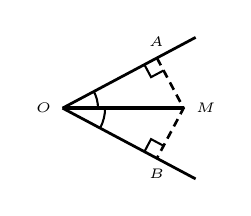
\begin{tikzpicture}[scale=0.58, every node/.style={font=\tiny, text=black}]
          \coordinate (O) at (0,0);
          \coordinate (X) at (28:3.3);
          \coordinate (Y) at (-28:3.3);
          \coordinate (M) at (0:2.65);
          \coordinate (A) at (28:2.34);
          \coordinate (B) at (-28:2.34);
          \draw[black, line width=1.0pt] (O) -- (X) (O) -- (Y);
          \draw[black, line width=1.4pt] (O) -- (M);
          \draw[black, densely dashed, line width=0.95pt] (A) -- (M) -- (B);
          \pic[draw=black, line width=0.75pt, angle radius=1.8mm]{right angle=O--A--M};
          \pic[draw=black, line width=0.75pt, angle radius=1.8mm]{right angle=O--B--M};
          \pic[draw=black, line width=0.75pt, angle radius=4.5mm]{angle=M--O--X};
          \pic[draw=black, line width=0.75pt, angle radius=5.4mm]{angle=Y--O--M};
          \node[left=0.5pt] at (O) {$O$}; \node[above=0.5pt] at (A) {$A$};
          \node[below=0.5pt] at (B) {$B$}; \node[right=1pt] at (M) {$M$};
        \end{tikzpicture}
      \end{minipage}
    \end{tcolorbox}
  \end{minipage}

  \vspace{3.5pt}

  % --- ផ្នែកទី ៣៖ តារាងធនាគារអំណះអំណាង ①–⑤ (អ.ម / HA) ---
  \fontsize{7.85pt}{10.9pt}\selectfont
  \renewcommand{\arraystretch}{1.06}
  \begin{tabular}{|C{0.70cm}|L{4.00cm}|L{6.55cm}|C{4.95cm}|}
    \hline
    \cellcolor{headgray}\textbf{លេខ} &
    \cellcolor{headgray}\centering\arraybackslash\textbf{ឈ្មោះអំណះអំណាង} &
    \cellcolor{headgray}\centering\arraybackslash\textbf{និមិត្តសញ្ញា និងរបៀបប្រើ} &
    \cellcolor{headgray}\centering\arraybackslash\textbf{រូបសម្គាល់ ស-ខ្មៅ} \\ \hline

    \cnum{1} &
    \textbf{បម្រាប់ / មុំកែង $90^\circ$} &
    មុំកែងប្រធាន៖ $\ang{A}=\ang{A'}=90^\circ$, $MA\perp OX$, $BD\perp AC$~។ &
    \raisebox{-0.35\height}{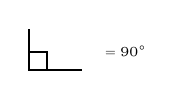
\begin{tikzpicture}[scale=0.52, every node/.style={font=\tiny, text=black}]
      \coordinate (o) at (0,0); \coordinate (a) at (1.3,0); \coordinate (b) at (0,1.0);
      \draw[black, line width=1.0pt] (b) -- (o) -- (a);
      \pic[draw=black, line width=0.8pt, angle radius=2.3mm]{right angle=a--o--b};
      \node[right=2pt] at (1.5,0.45) {$=90^\circ$};
    \end{tikzpicture}} \\ \hline

    \cnum{2} &
    \textbf{មុំស្រួចស្មើ}\newline (ពុះមុំ / $90^\circ-\text{មុំ}$) &
    $\ang{MOA}=\ang{MOB}$ (ពុះមុំ), មុំរួម $\ang{A}$, មុំបាតសមបាទ ឬ $90^\circ-\ang{C}$~។ &
    \raisebox{-0.35\height}{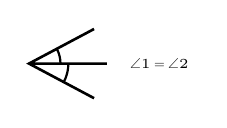
\begin{tikzpicture}[scale=0.52, every node/.style={font=\tiny, text=black}]
      \coordinate (o) at (0,0); \coordinate (x) at (28:1.8); \coordinate (m) at (0:1.9); \coordinate (y) at (-28:1.8);
      \draw[black, line width=0.95pt] (x)--(o)--(y) (o)--(m);
      \pic[draw=black, line width=0.8pt, angle radius=4.0mm]{angle=m--o--x};
      \pic[draw=black, line width=0.8pt, angle radius=5.0mm]{angle=y--o--m};
      \node[right=2pt] at (2.1, 0) {$\ang{1}=\ang{2}$};
    \end{tikzpicture}} \\ \hline

    \cnum{3} &
    \textbf{អ៊ីប៉ូតេនុសស្មើ ឬរួម}\newline (ឈម $90^\circ$) &
    ជ្រុងឈមមុំកែង $90^\circ$៖ $BC=B'C'$, $AB=AC$ ឬអ៊ីប៉ូតេនុសរួម $OM=OM$~។ &
    \raisebox{-0.35\height}{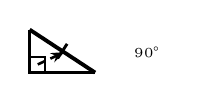
\begin{tikzpicture}[scale=0.52, every node/.style={font=\tiny, text=black}]
      \coordinate (a) at (0,0); \coordinate (b) at (1.6,0); \coordinate (c) at (0,1.05);
      \draw[black, line width=0.9pt] (c)--(a)--(b);
      \draw[black, line width=1.4pt, tk1] (b)--(c);
      \pic[draw=black, line width=0.8pt, angle radius=2.0mm]{right angle=b--a--c};
      \draw[hypArrow] (0.20,0.20) -- (0.85,0.50);
      \node[right=2pt] at (1.85,0.50) {ឈម $90^\circ$};
    \end{tikzpicture}} \\ \hline

    \cnum{4} &
    \textbf{លក្ខខណ្ឌ អ.ម (\en{HA})} &
    អ៊ីប៉ូតេនុសប៉ុនគ្នា $+$ មុំស្រួច ១ ប៉ុនគ្នា $\Rightarrow \tri{ABC}\cg\tri{A'B'C'}$~។ &
    \raisebox{-0.35\height}{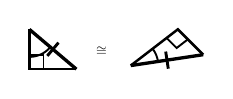
\begin{tikzpicture}[scale=0.46, every node/.style={font=\tiny, text=black}]
      \coordinate (a) at (0,0); \coordinate (b) at (1.3,0); \coordinate (c) at (0,1.1);
      \draw[black, line width=0.9pt] (c)--(a)--(b); \draw[black, line width=1.2pt, tk1] (b)--(c);
      \pic[draw=black, line width=0.7pt, angle radius=1.8mm]{right angle=b--a--c};
      \pic[draw=black, line width=0.7pt, angle radius=3.5mm]{angle=a--c--b};
      \node at (2.0,0.5) {$\cg$};
      \coordinate (d) at (4.1,1.1); \coordinate (e) at (4.8,0.4); \coordinate (f) at (2.8,0.1);
      \draw[black, line width=0.9pt] (f)--(d)--(e); \draw[black, line width=1.2pt, tk1] (e)--(f);
      \pic[draw=black, line width=0.7pt, angle radius=1.8mm]{right angle=f--d--e};
      \pic[draw=black, line width=0.7pt, angle radius=3.5mm]{angle=e--f--d};
    \end{tikzpicture}} \\ \hline

    \cnum{5} &
    \textbf{ធាតុត្រូវគ្នា / ចម្ងាយកែងស្មើ} &
    $MA=MB,\; BD=CE,\; AD=AE \Rightarrow BE=AB-AE=AC-AD=CD$~។ &
    \raisebox{-0.35\height}{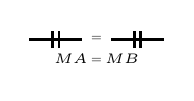
\begin{tikzpicture}[scale=0.52, every node/.style={font=\tiny, text=black}]
      \draw[black, line width=1.1pt, tk2] (0,0.2) -- (1.3,0.2);
      \node at (1.65,0.2) {$=$};
      \draw[black, line width=1.1pt, tk2] (2.0,0.2) -- (3.3,0.2);
      \node[below=1pt] at (1.65,0.15) {$MA=MB$};
    \end{tikzpicture}} \\ \hline
  \end{tabular}

  \vspace{3.5pt}

  % --- ផ្នែកទី ៤៖ ប្រអប់ព្រមាន "អន្ទាក់អ៊ីប៉ូតេនុស vs ជ្រុងកែង" & "អន្ទាក់ចម្ងាយទ្រេត (មិនកែង)" ---
  \noindent
  \begin{minipage}[t]{8.75cm}
    \begin{tcolorbox}[
      enhanced, sharp corners, colback=white, colframe=black,
      boxrule=1.15pt, boxsep=1pt, equal height group=posterwarnHA,
      top=3pt, bottom=3pt, left=5pt, right=5pt,
      title={\ding{55}\ \textbf{អន្ទាក់ទី ១៖ អ៊ីប៉ូតេនុស \en{vs} ជ្រុងកែង (\en{Hyp vs Leg})}},
      colbacktitle=midgray, coltitle=black, fonttitle=\fontsize{8.2pt}{11.2pt}\selectfont
    ]
      \centering
      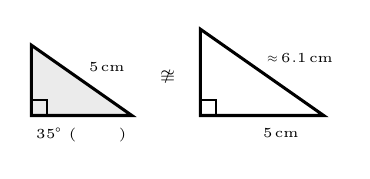
\begin{tikzpicture}[scale=0.58, every node/.style={font=\scriptsize, text=black}]
        \coordinate (P) at (0,0); \coordinate (R) at (2.2,0); \coordinate (Q) at (0,1.54);
        \fill[panelgray] (P)--(Q)--(R)--cycle;
        \draw[black, line width=1.1pt] (P)--(Q)--(R)--cycle;
        \pic[draw=black, line width=0.8pt, angle radius=2.0mm]{right angle=R--P--Q};
        \node[above right=0pt, font=\tiny] at (1.05,0.75) {$5\unit{cm}$};
        \node[below=1pt, font=\tiny] at (1.1,0) {$35^\circ$ (អ៊ីប៉ូតេនុស)};
        \node[font=\scriptsize] at (3.0, 0.85) {$\ncg$};
        \coordinate (Pp) at (3.7,0); \coordinate (Rp) at (6.4,0); \coordinate (Qp) at (3.7,1.89);
        \fill[white] (Pp)--(Qp)--(Rp)--cycle;
        \draw[black, line width=1.1pt] (Pp)--(Qp)--(Rp)--cycle;
        \pic[draw=black, line width=0.8pt, angle radius=2.0mm]{right angle=Rp--Pp--Qp};
        \node[below=1pt, font=\tiny] at (5.05,0) {ជ្រុងកែង $5\unit{cm}$};
        \node[above right=0pt, font=\tiny] at (4.95,0.95) {$\approx 6.1\unit{cm}$};
      \end{tikzpicture}
      \par\vspace{1.5pt}\fontsize{7.65pt}{10.8pt}\selectfont
      $5\unit{cm}$ នៅលើ\textbf{អ៊ីប៉ូតេនុស} ទល់ $5\unit{cm}$ នៅលើ\textbf{ជ្រុងកែង} មិនមែនលក្ខខណ្ឌ \textbf{អ.ម (\en{HA})} ទេ ($\tri{PQR}\ncg\tri{P'Q'R'}$)!
    \end{tcolorbox}
  \end{minipage}\hfill
  \begin{minipage}[t]{8.75cm}
    \begin{tcolorbox}[
      enhanced, sharp corners, colback=white, colframe=black,
      boxrule=1.15pt, boxsep=1pt, equal height group=posterwarnHA,
      top=3pt, bottom=3pt, left=5pt, right=5pt,
      title={\ding{55}\ \textbf{អន្ទាក់ទី ២៖ ចម្ងាយទ្រេត (មិនកែង) \en{\&} \tickone\ លើ $OA, OB$}},
      colbacktitle=midgray, coltitle=black, fonttitle=\fontsize{8.2pt}{11.2pt}\selectfont
    ]
      \centering
      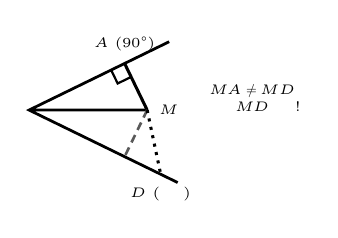
\begin{tikzpicture}[scale=0.60, every node/.style={font=\scriptsize, text=black}]
        \coordinate (O) at (0,0); \coordinate (X) at (26:3.3); \coordinate (Y) at (-26:3.5);
        \coordinate (M) at (0:2.5); \coordinate (A) at (26:2.25); \coordinate (B) at (-26:2.25); \coordinate (D) at (-26:3.1);
        \draw[black, line width=1.0pt] (X)--(O)--(Y) (O)--(M);
        \draw[black, line width=1.1pt] (M)--(A);
        \draw[darkline, densely dashed, line width=0.95pt] (M)--(B);
        \draw[black, dotted, line width=1.1pt] (M)--(D);
        \pic[draw=black, line width=0.8pt, angle radius=1.9mm]{right angle=O--A--M};
        \node[above=1pt, font=\tiny] at (A) {$A$ ($90^\circ$)};
        \node[below=1pt, font=\tiny] at (D) {$D$ (មិនកែង)};
        \node[right=1pt, font=\tiny] at (M) {$M$};
        \node[right=2pt, font=\tiny, align=left] at (3.5, 0.25) {$MA \neq MD$\\ព្រោះ $MD$ ទ្រេត!};
      \end{tikzpicture}
      \par\vspace{1.5pt}\fontsize{7.65pt}{10.8pt}\selectfont
      ចម្ងាយពី $M$ ទៅ $OX, OY$ ត្រូវវាស់តាមបន្ទាត់\textbf{កែង $90^\circ$} តែប៉ុណ្ណោះ (និង\textbf{ហាមបន្ថែម \tickone\ លើ $OA=OB$})!
    \end{tcolorbox}
  \end{minipage}
\end{tcolorbox}

\clearpage

% ============================================================================
% ទំព័រទី ៥៖ កាតវិនិច្ឆ័យរហ័ស ៦០–៩០ វិនាទី "កាត A–D" & តារាងចម្លើយគ្រូ — E5 Evaluate
% ============================================================================
\pagebanner{សម្ភារៈទី ៥៖ កាតវិនិច្ឆ័យរហ័ស «កាត \enbf{A--D}» \enbf{(60--90} វិនាទី\enbf{) \&} ចម្លើយគ្រូ}{ទំព័រ ៥/៦ \en{-- E5 Evaluate}}

{\fontsize{8.5pt}{12pt}\selectfont
\textbf{វិធីលេងក្នុងថ្នាក់៖} គ្រូលើកកាតម្ដងមួយ $\rightarrow$ សិស្សចង្អុលប្រអប់ $90^\circ$ ទៅអ៊ីប៉ូតេនុស $\rightarrow$ លើក \textbf{មេដៃឡើង (ពិត \ding{51})} ឬ \textbf{ខ្វែងដៃ (ខុស/អន្ទាក់ \ding{55})} + ម្រាម \en{1--3}។}

\vspace{4pt}

% --- ជួរទី ១៖ កាត A & កាត B ---
\noindent
\begin{tcolorbox}[
  enhanced, sharp corners, colback=white, colframe=white,
  borderline={1.0pt}{0pt}{black, dashed},
  width=9.25cm, equal height group=hafoilrow1, nobeforeafter,
  boxsep=1pt, top=5pt, bottom=5pt, left=6pt, right=6pt
]
  \noindent\colorbox{black}{\textcolor{white}{\Large\textbf{\en{ A }}}}\hspace{0.25cm}{\fontsize{9.2pt}{12.5pt}\selectfont\textbf{កាត \en{A} ៖ អ.ម (\en{HA}) បង្វិល $\approx 135^\circ$}}\par\vspace{2pt}
  \begin{center}
  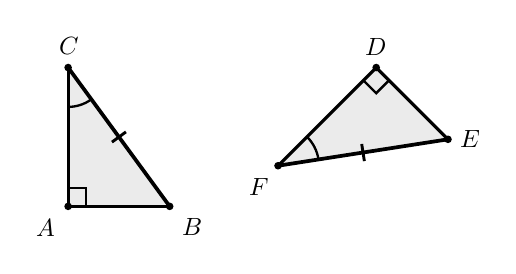
\begin{tikzpicture}[scale=0.86, every node/.style={font=\small, text=black}]
    % Upright ∆ABC
    \coordinate (A) at (0,0); \coordinate (B) at (1.50,0); \coordinate (C) at (0, 2.05);
    \fill[panelgray] (A)--(B)--(C)--cycle;
    \draw[black, line width=1.15pt] (C)--(A)--(B);
    \draw[black, line width=1.35pt, tk1] (B)--(C);
    \pic[draw=black, line width=0.85pt, angle radius=2.3mm]{right angle=B--A--C};
    \pic[draw=black, line width=0.85pt, angle radius=5.0mm]{angle=A--C--B};
    \fill[black] (A) circle (1.6pt) (B) circle (1.6pt) (C) circle (1.6pt);
    \node[below left=1pt] at (A) {$A$}; \node[below right=1pt] at (B) {$B$}; \node[above=1pt] at (C) {$C$};
    % បង្វិល ~135° ∆DEF
    \coordinate (D) at (4.55, 2.05); \coordinate (E) at (5.61, 0.99); \coordinate (F) at (3.10, 0.60);
    \fill[panelgray] (D)--(E)--(F)--cycle;
    \draw[black, line width=1.15pt] (F)--(D)--(E);
    \draw[black, line width=1.35pt, tk1] (E)--(F);
    \pic[draw=black, line width=0.85pt, angle radius=2.3mm]{right angle=F--D--E};
    \pic[draw=black, line width=0.85pt, angle radius=5.2mm]{angle=E--F--D};
    \fill[black] (D) circle (1.6pt) (E) circle (1.6pt) (F) circle (1.6pt);
    \node[above=1pt] at (D) {$D$}; \node[right=1pt] at (E) {$E$}; \node[below left=1pt] at (F) {$F$};
  \end{tikzpicture}
  \end{center}
  {\centering\fontsize{8.0pt}{11pt}\selectfont $\ang{A}=\ang{D}=90^\circ$, $BC=EF$, $\ang{C}=\ang{F}$~។\par}
  \vfill
  \begin{tcolorbox}[enhanced, sharp corners, colback=panelgray, colframe=black, boxrule=0.8pt, boxsep=1pt, top=4pt, bottom=4pt, left=5pt, right=5pt]
    \centering\fontsize{9.0pt}{12.5pt}\selectfont
    \textbf{សំណួរ៖} តើ $\tri{ABC} \cg \tri{DEF}$ តាម \textbf{អ.ម (\en{HA})} ឬទេ?\\[2pt]
    \chkbox\ មេដៃឡើង (\ding{51} ពិត) \hspace{0.4cm} \chkbox\ ខ្វែងដៃ (\ding{55} ខុស)
  \end{tcolorbox}
\end{tcolorbox}%
\hfill
\begin{tcolorbox}[
  enhanced, sharp corners, colback=white, colframe=white,
  borderline={1.0pt}{0pt}{black, dashed},
  width=9.25cm, equal height group=hafoilrow1, nobeforeafter,
  boxsep=1pt, top=5pt, bottom=5pt, left=6pt, right=6pt
]
  \noindent\colorbox{black}{\textcolor{white}{\Large\textbf{\en{ B }}}}\hspace{0.25cm}{\fontsize{9.2pt}{12.5pt}\selectfont\textbf{កាត \en{B} ៖ អន្ទាក់អ៊ីប៉ូតេនុស $5\unit{cm}$ \en{vs} ជ្រុងកែង $5\unit{cm}$}}\par\vspace{2pt}
  \begin{center}
  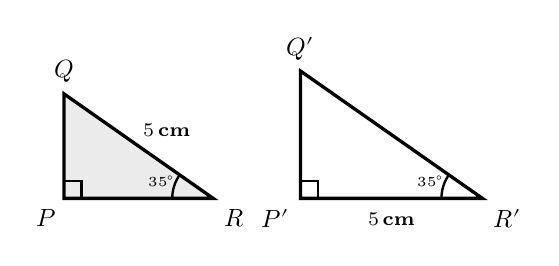
\begin{tikzpicture}[scale=0.66, every node/.style={font=\small, text=black}]
    % PQR hyp=5cm
    \coordinate (P) at (0,0); \coordinate (R) at (2.87,0); \coordinate (Q) at (0, 2.01);
    \fill[panelgray] (P)--(Q)--(R)--cycle;
    \draw[black, line width=1.2pt] (P)--(Q)--(R)--cycle;
    \pic[draw=black, line width=0.85pt, angle radius=2.2mm]{right angle=R--P--Q};
    \pic[draw=black, line width=0.85pt, angle radius=5.2mm]{angle=Q--R--P};
    \node[font=\tiny] at ($(R)+(162:1.05)$) {$35^\circ$};
    \node[above right=0pt, font=\scriptsize] at (1.35, 1.00) {\textbf{$5\unit{cm}$}};
    \node[below left=0.5pt] at (P) {$P$}; \node[above=0.5pt] at (Q) {$Q$}; \node[below right=0.5pt] at (R) {$R$};
    % P'Q'R' leg=5cm (shifted right cleanly to 4.55)
    \coordinate (Pp) at (4.55,0); \coordinate (Rp) at (8.05,0); \coordinate (Qp) at (4.55, 2.45);
    \fill[white] (Pp)--(Qp)--(Rp)--cycle;
    \draw[black, line width=1.2pt] (Pp)--(Qp)--(Rp)--cycle;
    \pic[draw=black, line width=0.85pt, angle radius=2.2mm]{right angle=Rp--Pp--Qp};
    \pic[draw=black, line width=0.85pt, angle radius=5.2mm]{angle=Qp--Rp--Pp};
    \node[font=\tiny] at ($(Rp)+(162:1.05)$) {$35^\circ$};
    \node[below=1.5pt, font=\scriptsize] at (6.30, 0) {\textbf{$5\unit{cm}$}};
    \node[below left=0.5pt] at (Pp) {$P'$}; \node[above=0.5pt] at (Qp) {$Q'$}; \node[below right=0.5pt] at (Rp) {$R'$};
  \end{tikzpicture}
  \end{center}
  {\centering\fontsize{8.0pt}{11pt}\selectfont មាន $90^\circ, 35^\circ$ និង $QR=5\unit{cm}$ ទល់ $P'R'=5\unit{cm}$~។\par}
  \vfill
  \begin{tcolorbox}[enhanced, sharp corners, colback=panelgray, colframe=black, boxrule=0.8pt, boxsep=1pt, top=4pt, bottom=4pt, left=5pt, right=5pt]
    \centering\fontsize{9.0pt}{12.5pt}\selectfont
    \textbf{សំណួរ៖} តើ $\tri{PQR} \cg \tri{P'Q'R'}$ តាម \textbf{អ.ម (\en{HA})} ឬទេ?\\[2pt]
    \chkbox\ មេដៃឡើង (\ding{51} ពិត) \hspace{0.4cm} \chkbox\ ខ្វែងដៃ (\ding{55} ខុស)
  \end{tcolorbox}
\end{tcolorbox}

\vspace{6pt}

% --- ជួរទី ២៖ កាត C & កាត D ---
\noindent
\begin{tcolorbox}[
  enhanced, sharp corners, colback=white, colframe=white,
  borderline={1.0pt}{0pt}{black, dashed},
  width=9.25cm, equal height group=hafoilrow2, nobeforeafter,
  boxsep=1pt, top=5pt, bottom=5pt, left=6pt, right=6pt
]
  \noindent\colorbox{black}{\textcolor{white}{\Large\textbf{\en{ C }}}}\hspace{0.25cm}{\fontsize{9.2pt}{12.5pt}\selectfont\textbf{កាត \en{C} ៖ អន្ទាក់អង្កត់ទ្រេត $MD$ មិនកែង $OY$}}\par\vspace{2pt}
  \begin{center}
  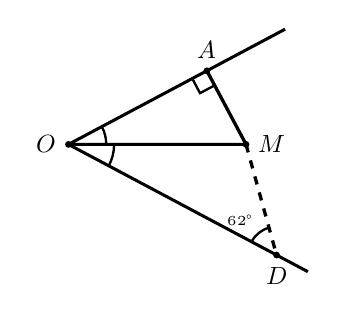
\begin{tikzpicture}[scale=0.82, every node/.style={font=\small, text=black}]
    \coordinate (O) at (0,0); \coordinate (X) at (28:3.8); \coordinate (Y) at (-28:4.2);
    \coordinate (M) at (0:2.75);
    \coordinate (A) at (28:2.428);
    \coordinate (D) at (-28:3.65); % slanted decoy!
    \draw[black, line width=1.1pt] (X)--(O)--(Y) (O)--(M);
    \draw[black, line width=1.2pt] (M)--(A);
    \draw[black, line width=1.2pt, dashed] (M)--(D);
    \pic[draw=black, line width=0.85pt, angle radius=2.1mm]{right angle=O--A--M};
    \pic[draw=black, line width=0.85pt, angle radius=4.8mm]{angle=M--O--X};
    \pic[draw=black, line width=0.85pt, angle radius=5.8mm]{angle=Y--O--M};
    \pic[draw=black, line width=0.85pt, angle radius=3.6mm]{angle=M--D--O};
    \node[font=\tiny] at ($(D)+(136:0.78)$) {$62^\circ$};
    \fill[black] (O) circle (1.5pt) node[left=1pt] {$O$};
    \fill[black] (A) circle (1.5pt) node[above=1pt] {$A$};
    \fill[black] (M) circle (1.5pt) node[right=1pt] {$M$};
    \fill[black] (D) circle (1.5pt) node[below=1pt] {$D$};
  \end{tikzpicture}
  \end{center}
  {\centering\fontsize{8.0pt}{11pt}\selectfont $OM$ ពុះ $\ang{XOY}$, $MA\perp OX$ តែ $MD$ ទ្រេត ($\ang{MDO}=62^\circ$)~។\par}
  \vfill
  \begin{tcolorbox}[enhanced, sharp corners, colback=panelgray, colframe=black, boxrule=0.8pt, boxsep=1pt, top=4pt, bottom=4pt, left=5pt, right=5pt]
    \centering\fontsize{9.0pt}{12.5pt}\selectfont
    \textbf{សំណួរ៖} គេថា $MA = MD$ តាមលក្ខណៈពុះមុំ ត្រូវឬខុស?\\[2pt]
    \chkbox\ មេដៃឡើង (\ding{51} ពិត) \hspace{0.4cm} \chkbox\ ខ្វែងដៃ (\ding{55} ខុស)
  \end{tcolorbox}
\end{tcolorbox}%
\hfill
\begin{tcolorbox}[
  enhanced, sharp corners, colback=white, colframe=white,
  borderline={1.0pt}{0pt}{black, dashed},
  width=9.25cm, equal height group=hafoilrow2, nobeforeafter,
  boxsep=1pt, top=5pt, bottom=5pt, left=6pt, right=6pt
]
  \noindent\colorbox{black}{\textcolor{white}{\Large\textbf{\en{ D }}}}\hspace{0.25cm}{\fontsize{9.2pt}{12.5pt}\selectfont\textbf{កាត \en{D} ៖ អន្ទាក់ \en{AA} ($90^\circ, 35^\circ$ គ្មានអ៊ីប៉ូតេនុស)}}\par\vspace{2pt}
  \begin{center}
  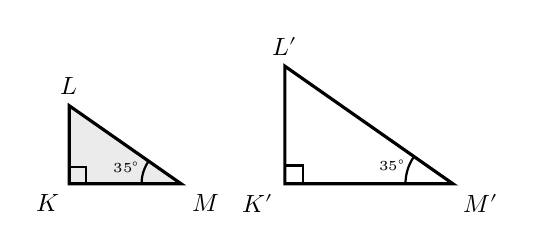
\begin{tikzpicture}[scale=0.66, every node/.style={font=\small, text=black}]
    % Small KLM
    \coordinate (K) at (0,0); \coordinate (M) at (2.15,0); \coordinate (L) at (0, 1.50);
    \fill[panelgray] (K)--(L)--(M)--cycle;
    \draw[black, line width=1.15pt] (K)--(L)--(M)--cycle;
    \pic[draw=black, line width=0.8pt, angle radius=2.1mm]{right angle=M--K--L};
    \pic[draw=black, line width=0.8pt, angle radius=5.0mm]{angle=L--M--K};
    \node[font=\tiny] at ($(M)+(163:1.10)$) {$35^\circ$};
    \node[below left=0.5pt] at (K) {$K$}; \node[above=0.5pt] at (L) {$L$}; \node[below right=0.5pt] at (M) {$M$};
    % Larger K'L'M' (shifted right cleanly to 4.15)
    \coordinate (Kp) at (4.15,0); \coordinate (Mp) at (7.38,0); \coordinate (Lp) at (4.15, 2.26);
    \fill[white] (Kp)--(Lp)--(Mp)--cycle;
    \draw[black, line width=1.15pt] (Kp)--(Lp)--(Mp)--cycle;
    \pic[draw=black, line width=0.8pt, angle radius=2.3mm]{right angle=Mp--Kp--Lp};
    \pic[draw=black, line width=0.8pt, angle radius=6.0mm]{angle=Lp--Mp--Kp};
    \node[font=\tiny] at ($(Mp)+(163:1.22)$) {$35^\circ$};
    \node[below left=0.5pt] at (Kp) {$K'$}; \node[above=0.5pt] at (Lp) {$L'$}; \node[below right=0.5pt] at (Mp) {$M'$};
  \end{tikzpicture}
  \end{center}
  {\centering\fontsize{8.0pt}{11pt}\selectfont មាន $\ang{K}=\ang{K'}=90^\circ$ និង $\ang{M}=\ang{M'}=35^\circ$ (គ្មានប្រវែងជ្រុង)~។\par}
  \vfill
  \begin{tcolorbox}[enhanced, sharp corners, colback=panelgray, colframe=black, boxrule=0.8pt, boxsep=1pt, top=4pt, bottom=4pt, left=5pt, right=5pt]
    \centering\fontsize{9.0pt}{12.5pt}\selectfont
    \textbf{សំណួរ៖} មុំ ២ គូស្មើ ($90^\circ, 35^\circ$) តើ $\tri{KLM}\cg\tri{K'L'M'}$ ទេ?\\[2pt]
    \chkbox\ មេដៃឡើង (\ding{51} ពិត) \hspace{0.4cm} \chkbox\ ខ្វែងដៃ (\ding{55} ខុស)
  \end{tcolorbox}
\end{tcolorbox}

\vspace{6pt}

% --- ខ្សែកាត់ & បន្ទះចម្លើយសម្រាប់គ្រូ ---
\noindent\scissors\ \dotfill\ \textbf{កាត់ទុកសម្រាប់គ្រូ (\en{Teacher Mini Answer \& Remediation Key})} \dotfill\ \scissors

\vspace{4pt}
\begin{tcolorbox}[
  enhanced, sharp corners, colback=panelgray, colframe=black,
  boxrule=1.0pt, boxsep=1pt, top=4pt, bottom=4pt, left=5pt, right=5pt
]
  \fontsize{7.75pt}{10.9pt}\selectfont
  \renewcommand{\arraystretch}{1.10}
  \begin{tabular}{|L{4.05cm}|L{4.25cm}|L{4.25cm}|L{4.45cm}|}
    \hline
    \cellcolor{headgray}\textbf{កាត \en{A} ៖ មេដៃឡើង (\ding{51})} &
    \cellcolor{headgray}\textbf{កាត \en{B} ៖ ខ្វែងដៃ (\ding{55})} &
    \cellcolor{headgray}\textbf{កាត \en{C} ៖ ខ្វែងដៃ (\ding{55})} &
    \cellcolor{headgray}\textbf{កាត \en{D} ៖ ខ្វែងដៃ (\ding{55})} \\ \hline
    $\tri{ABC}\cg\tri{DEF}$ តាម \textbf{អ.ម (\en{HA})} ទោះបង្វិល $\approx 135^\circ$ ព្រោះ $90^\circ$, អ៊ីប៉ូតេនុស $BC=EF$, មុំស្រួច $\ang{C}=\ang{F}$! &
    \textbf{អន្ទាក់អ៊ីប៉ូតេនុស \en{vs} ជ្រុងកែង!} $QR=5\unit{cm}$ ឈម $90^\circ$ តែ $P'R'=5\unit{cm}$ ជាជ្រុងកែង ($Q'R'\approx 6.1\unit{cm} \Rightarrow \ncg$)។ &
    \textbf{ចម្ងាយទ្រេត មិនកែង!} $MD$ មិនកែង $OY$ ($\ang{MDO}=62^\circ \neq 90^\circ$) ដូច្នេះ $MD > MA$ មិនមែនចម្ងាយកែងទេ។ &
    \textbf{អន្ទាក់ \en{AA} (គ្មានជ្រុង)!} $90^\circ, 35^\circ$ ធ្វើឱ្យរូបដូចគ្នា តែគ្មានអ៊ីប៉ូតេនុសប៉ុនគ្នា ($\tri{KLM}\ncg\tri{K'L'M'}$)! \\ \hline
  \end{tabular}
  \par\vspace{2.5pt}
  \textbf{ត្រួតទំនុកចិត្ត (ម្រាម ១\en{--}៣)៖} ១ ម្រាម = គូសព្រួញ $90^\circ \to$ អ៊ីប៉ូតេនុសជាមួយដៃគូ \hspace{0.2cm}\en{|}\hspace{0.2cm} ២ ម្រាម = ផ្ទៀងធនាគារ \cnum{1}--\cnum{5} \hspace{0.2cm}\en{|}\hspace{0.2cm} ៣ ម្រាម = ច្បាស់ ១០០\%
\end{tcolorbox}

\clearpage

% ============================================================================
% ទំព័រទី ៦៖ ប័ណ្ណកិច្ចការផ្ទះ ជំហានទី ៥ — ៤ ប័ណ្ណក្នុង ១ ទំព័រ A4 (4-up: HW #6 & #7)
% ============================================================================
\pagebanner{សម្ភារៈទី ៦៖ ប័ណ្ណកិច្ចការផ្ទះ ជំហានទី ៥ \enbf{--} ៤ ប័ណ្ណក្នុង ១ ទំព័រ \enbf{A4}}{ទំព័រ ៦/៦ \en{--} ជំហានទី ៥ (កាត់ ៤ ប័ណ្ណ \scissors)}

% ម៉ាក្រូប័ណ្ណកិច្ចការផ្ទះ ៤-up (ផ្ទៀង ១០០% នឹងលំហាត់ទី ៦ ទំព័រ ១៦៤ និងលំហាត់ទី ៧ ទំព័រ ១៦៥)
\newcommand{\hwslipFourHA}[1]{%
\begin{tcolorbox}[
  enhanced, sharp corners, colback=white, colframe=white,
  borderline={0.95pt}{0pt}{black, dashed},
  width=9.25cm, equal height group=hwquadHA, nobeforeafter,
  boxsep=1pt, top=3.5pt, bottom=3.5pt, left=4.5pt, right=4.5pt
]
  \begin{tcolorbox}[
    enhanced, sharp corners, colback=headgray, colframe=black,
    boxrule=0.7pt, boxsep=1pt, top=2pt, bottom=2pt, left=4pt, right=4pt, after skip=4pt
  ]
    \fontsize{7.55pt}{10.5pt}\selectfont
    \textbf{\scissors\ កិច្ចការផ្ទះ (#1) \en{|} ១.៣.១ អ.ម (\en{HA}) \& ពុះមុំ} \hfill \textbf{សៅរ៍ ២៨/១១/២៦}\\[1.5pt]
    ឈ្មោះ៖ $\underline{\hspace{4.0cm}}$ \hspace{0.2cm} ថ្នាក់៖ $\underline{\hspace{1.0cm}}$
  \end{tcolorbox}

  % --- លំហាត់ទី ៦ (សៀវភៅទំព័រ ១៦៤) ---
  \noindent
  \begin{minipage}[c]{5.25cm}
    \fontsize{7.5pt}{10.8pt}\selectfont
    \textbf{លំហាត់ទី ៦ (ទំ.១៦៤)៖} គេឱ្យ $\ang{BAD}=\ang{CAD}$ និង $AD\perp BC$~។ បង្ហាញថា $\tri{ABD}\cg\tri{ACD}$ និង $AB=AC$~។\\
    {\fontsize{6.8pt}{9.6pt}\selectfont\textit{តម្រុយ៖} $AD$ ជា\textbf{ជ្រុងជាប់កែងរួម} (មិនមែនអ៊ីប៉ូតេនុស!) $\Rightarrow$ ស្រាយតាម \textbf{ម.ជ.ម (\en{ASA})}!}
  \end{minipage}\hfill
  \begin{minipage}[c]{3.15cm}
    \centering
    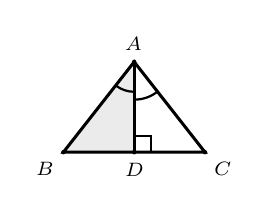
\begin{tikzpicture}[scale=0.62, every node/.style={font=\scriptsize, text=black}]
      % Ex. #6 (Book p. 164)
      \coordinate (A) at (0, 1.85);
      \coordinate (B) at (-1.45, 0);
      \coordinate (C) at (1.45, 0);
      \coordinate (D) at (0, 0);
      \fill[panelgray] (A) -- (B) -- (D) -- cycle;
      \draw[black, line width=1.1pt] (A) -- (B) -- (C) -- cycle;
      \draw[black, line width=1.15pt] (A) -- (D);
      \pic[draw=black, line width=0.8pt, angle radius=2.1mm]{right angle=A--D--C};
      \pic[draw=black, line width=0.8pt, angle radius=3.8mm]{angle=B--A--D};
      \pic[draw=black, line width=0.8pt, angle radius=4.8mm]{angle=D--A--C};
      \fill[black] (A) circle (1.3pt) node[above=0.5pt] {$A$};
      \fill[black] (B) circle (1.3pt) node[below left=0pt] {$B$};
      \fill[black] (C) circle (1.3pt) node[below right=0pt] {$C$};
      \fill[black] (D) circle (1.3pt) node[below=0.5pt] {$D$};
    \end{tikzpicture}
  \end{minipage}

  \vspace{4pt}
  \hrule height 0.5pt
  \vspace{4pt}

  % --- លំហាត់ទី ៧ (សៀវភៅទំព័រ ១៦៥) ---
  \noindent
  \begin{minipage}[c]{5.25cm}
    \fontsize{7.4pt}{10.7pt}\selectfont
    \textbf{លំហាត់ទី ៧ (ទំ.១៦៥)៖} $P$ លើកន្លះពុះ $\ang{A}$ នៃត្រីកោណសមបាទ $ABC$ ($AB=AC$)~។\\
    \textbf{ក.} ស្រាយថា $PB=PC$ (\textbf{ជ.ម.ជ})~។\\
    \textbf{ខ.} គូសបន្ថែម $PH\perp AB, PK\perp AC \Rightarrow PH=PK$ (ដោយ \textbf{អ.ម})~។
  \end{minipage}\hfill
  \begin{minipage}[c]{3.15cm}
    \centering
    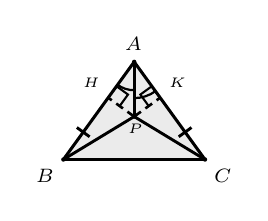
\begin{tikzpicture}[scale=0.62, every node/.style={font=\scriptsize, text=black}]
      % Ex. #7 (Book p. 165) + extended perp feet H, K
      % Exact feet: A=(0,2.0), B=(-1.45,0), C=(1.45,0), P=(0,0.88) -> t = (1.12*2.0)/6.1025 = 0.36706
      % H=(-0.5322, 1.2659), K=(0.5322, 1.2659) — tk1low at 0.72 avoids H/K right-angle boxes!
      \coordinate (A) at (0, 2.0);
      \coordinate (B) at (-1.45, 0);
      \coordinate (C) at (1.45, 0);
      \coordinate (P) at (0, 0.88);
      \coordinate (H) at (-0.5322, 1.2659);
      \coordinate (K) at (0.5322, 1.2659);
      \fill[panelgray] (A) -- (B) -- (C) -- cycle;
      \draw[black, line width=1.1pt, tk1low] (A) -- (B);
      \draw[black, line width=1.1pt, tk1low] (A) -- (C);
      \draw[black, line width=1.05pt] (B) -- (C) (B) -- (P) -- (C);
      \draw[black, line width=1.15pt] (A) -- (P);
      \draw[black, densely dashed, line width=0.95pt] (P) -- (H) (P) -- (K);
      \pic[draw=black, line width=0.75pt, angle radius=1.8mm]{right angle=A--H--P};
      \pic[draw=black, line width=0.75pt, angle radius=1.8mm]{right angle=A--K--P};
      \pic[draw=black, line width=0.8pt, angle radius=3.6mm]{angle=B--A--P};
      \pic[draw=black, line width=0.8pt, angle radius=4.6mm]{angle=P--A--C};
      \fill[black] (A) circle (1.3pt) node[above=0.5pt] {$A$};
      \fill[black] (B) circle (1.3pt) node[below left=0pt] {$B$};
      \fill[black] (C) circle (1.3pt) node[below right=0pt] {$C$};
      \fill[black] (P) circle (1.3pt);
      \node[below=2pt, font=\tiny, fill=panelgray, inner sep=0.5pt] at (P) {$P$};
      \node[above left=0pt, font=\tiny] at (H) {$H$};
      \node[above right=0pt, font=\tiny] at (K) {$K$};
    \end{tikzpicture}
  \end{minipage}

  \vspace{4pt}
  \begin{tcolorbox}[
    enhanced, sharp corners, colback=panelgray, colframe=black,
    boxrule=0.75pt, boxsep=1pt, top=3pt, bottom=3pt, left=4pt, right=4pt
  ]
    \fontsize{7.05pt}{10.1pt}\selectfont
    \textbf{ផ្ទៀងខ្លួនឯង (\en{Warrant \cnum{1}--\cnum{5}})៖}
    \chkbox\ គូស $90^\circ$ ($AD\perp BC$ និង $PH\perp AB, PK\perp AC$) + ព្រួញអ៊ីប៉ូតេនុស!\\
    \chkbox\ បែងចែក \textbf{ម.ជ.ម} (លំ.៦) \en{|} \textbf{ជ.ម.ជ} (លំ.៧ក) \en{|} \textbf{អ.ម} (លំ.៧ខ $AP$ រួម)!\\
    \chkbox\ ដាក់លេខ \cnum{1}--\cnum{5} គ្រប់បន្ទាត់ និងប្រើ $=$ (ប្រវែង/មុំ) ទល់ $\cg$ (ត្រីកោណ)។
  \end{tcolorbox}
\end{tcolorbox}%
}

\noindent
\hwslipFourHA{ប័ណ្ណទី ១}\hfill\hwslipFourHA{ប័ណ្ណទី ២}

\vspace{7pt}
\noindent\scissors\ \dotfill\ \textbf{កាត់តាមស្នាមចុចចែកជា ៤ ប័ណ្ណ (\en{Cut Along Dashed Lines})} \dotfill\ \scissors
\vspace{7pt}

\noindent
\hwslipFourHA{ប័ណ្ណទី ៣}\hfill\hwslipFourHA{ប័ណ្ណទី ៤}

\end{document}
